%%%%%%%%%%%%%%%%%%%%%%%%%%%%%%%%%%%%%%%%%%%%%%%%%%%%%%%%%%
%
% eXascale Infolab thesis template -- Bachelor and Masters
% version 1.1, Oct 2019
%
%%%%%%%%%%%%%%%%%%%%%%%%%%%%%%%%%%%%%%%%%%%%%%%%%%%%%%%%%%
%
% Based on:
% Masters/Doctoral Thesis
% LaTeX Template Version 2.5 (27/8/17)
% http://www.LaTeXTemplates.com
% CC BY-NC-SA 3.0 (http://creativecommons.org/licenses/by-nc-sa/3.0/)
%
%%%%%%%%%%%%%%%%%%%%%%%%%%%%%%%%%%%%%%%%%

\documentclass[11pt,english,singlespacing,headsepline,consistentlayout]{structure/XI_thesis}

%----------------------------------------------------------------------------------------
%	LATEX PACKAGES
%----------------------------------------------------------------------------------------

%%%%%%%%%%%%%%%%%%%%%%%%%%% DO NOT EDIT
\usepackage[utf8]{inputenc} % Required for inputting international characters
\usepackage[T1]{fontenc} % Output font encoding for international characters
\usepackage{mathpazo} % Use the Palatino font by default
\usepackage[backend=bibtex,style=numeric,maxcitenames=2,natbib=true,sorting=none]{biblatex} % Use the bibtex backend with the authoryear citation style (which resembles APA)
\usepackage[autostyle=true]{csquotes} % Required to generate language-dependent quotes in the bibliography
\usepackage{booktabs}       % professional-quality tables
\usepackage{array}          % custom sizes for table columns
\usepackage{amssymb}        % extended blackboard math symbols
\usepackage{amsmath}        % complete AMS math package
% \usepackage[english]{babel} % spelling / syllabification
\usepackage{algorithm}      % pseudocode float
\usepackage[noend]{algpseudocode}  % pseudocode macros
\usepackage{graphicx}       % include graphics
\usepackage{epstopdf}       % vectorial graphics
\usepackage{subcaption}     % sub captions
\usepackage{url}            % URLs
%%%%%%%%%%%%%%%%%%%%%%%%%%% DO NOT EDIT - end

% Define path and extensions for your graphics
\graphicspath{{figures/}}%{{../jpeg/} [...]}
\DeclareGraphicsExtensions{.pdf,.jpg,.jpeg,.png,eps}


%% User packages
\usepackage{listings}
\usepackage{xcolor}
% Include your package settings in `structure/settings.tex`

%% User commands
\newcommand{\cb}[1]{\textcolor{red}{[#1]}}


% Load package settings
% !TEX root = ../main.tex

%----------------------------------------------------------------------------------------
% PACKAGE CONFIGURATIONS
%----------------------------------------------------------------------------------------

% Filename of the bibliography
\addbibresource{structure/main.bib}

% Margin settings
\geometry{
  paper=a4paper, % Paper format
  inner=2.5cm, % Inner margin
  outer=3.8cm, % Outer margin
  bindingoffset=.5cm, % Binding offset
  top=1.5cm, % Top margin
  bottom=1.5cm, % Bottom margin
  %showframe, % Uncomment to show how the type block is set on the page
}

% Figures location
\graphicspath{{figures/}}
\DeclareGraphicsExtensions{.pdf,.png,.jpg,.jpeg,.eps,.ps}

% Listings
% \definecolor{codegreen}{rgb}{0,0.6,0}
% \definecolor{codegray}{rgb}{0.5,0.5,0.5}
% \definecolor{codepurple}{rgb}{0.58,0,0.82}
% \definecolor{backcolour}{rgb}{0.95,0.95,0.92}
%
% \lstdefinestyle{mystyle}{
%     backgroundcolor=\color{backcolour},
%     commentstyle=\color{codegreen},
%     keywordstyle=\color{magenta},
%     numberstyle=\tiny\color{codegray},
%     stringstyle=\color{codepurple},
%     basicstyle=\ttfamily\footnotesize,
%     breakatwhitespace=false,
%     breaklines=true,
%     captionpos=b,
%     keepspaces=true,
%     numbers=left,
%     numbersep=5pt,
%     showspaces=false,
%     showstringspaces=false,
%     showtabs=false,
%     tabsize=2
% }
%
% \lstset{style=mystyle}

\definecolor{gray}{rgb}{0.4,0.4,0.4}
\definecolor{darkblue}{rgb}{0.0,0.0,0.6}
\definecolor{orangeweb}{rgb}{1,0.55,0}
\definecolor{darkgreen}{rgb}{0,0.55,0}
\definecolor{cyan}{rgb}{0.0,0.6,0.6}

\lstset{
  basicstyle=\ttfamily,
  columns=fullflexible,
  showstringspaces=false,
  commentstyle=\color{gray}\upshape
}

\lstdefinelanguage{XML}
{
  morestring=[b]",
  morestring=[s]{>}{<},
  morecomment=[s]{<?}{?>},
  stringstyle=\color{black},
  identifierstyle=\color{darkgreen},
  keywordstyle=\color{cyan},
  morekeywords={xmlns,version,type}% list your attributes here
}

% Load custom thesis information (remember to fill in)
% !TEX root = ../main.tex

%----------------------------------------------------------------------------------------
% THESIS INFORMATION
%----------------------------------------------------------------------------------------

% \thesistitle{Preprocessing New Datasets And Adding Segmentation To A Computer Aided Diagnosis System: The Hydra Model} % Your thesis title, this is used in the title and abstract, print it elsewhere with \ttitle
\thesistitle{Pre-Processing Segmentation Datasets for the Hydra Framework}
\supervisor{Prof. Dr. Philippe Cudré-Mauroux} % Your supervisor's name, this is used in the title page, print it elsewhere with \supname
\cosupervisor{Dr. Giuseppe Cuccu} % If you have a co-supervisor, include it here. This is used in the title page, print it elsewhere with \cosupname
\degree{Bachelor} % Your degree name, this is used in the title page and abstract, print it elsewhere with \degreename
\author{Christophe Broillet} % Your name, this is used in the title page and abstract, print it elsewhere with \authorname
\addresses{Bd de Pérolles 90} % Your address, this is not currently used anywhere in the template, print it elsewhere with \addressname

\subject{Computer Science} % Your subject area, this is not currently used anywhere in the template, print it elsewhere with \subjectname
\keywords{Machine Learning (ML), Deep Learning, Convolutional Neural Network (CNN), Computer Aided Diagnosis (CAD) System, Segmentation, Cancer} % Keywords for your thesis, this is not currently used anywhere in the template, print it elsewhere with \keywordnames
\university{\href{http://www.unifr.ch}{University of Fribourg}} % Your university's name and URL, this is used in the title page and abstract, print it elsewhere with \univname
\department{\href{https://www3.unifr.ch/inf/fr/}{Department of Informatics}} % Your department's name and URL, this is used in the title page and abstract, print it elsewhere with \deptname
\group{\href{https://www3.unifr.ch/inf/en/exascale-infolab.html}{eXascale Infolab}} % Your research group's name and URL, this is used in the title page, print it elsewhere with \groupname
\faculty{\href{https://www3.unifr.ch/scimed/fr/}{Faculty of Science and Medicine}} % Your faculty's name and URL, this is used in the title page and abstract, print it elsewhere with \facname

% Set title, author and keywords on the compiled PDF
\AtBeginDocument{
  \hypersetup{pdftitle=\ttitle} % Set the PDF's title to your title
  \hypersetup{pdfauthor=\authorname} % Set the PDF's author to your name
  \hypersetup{pdfkeywords=\keywordnames} % Set the PDF's keywords to your keywords
}

%----------------------------------------------------------------------------------------
\begin{document}
\frontmatter
\pagestyle{plain}
% Title page definition
% !TEX root = ../main.tex

%----------------------------------------------------------------------------------------
% TITLE PAGE
%----------------------------------------------------------------------------------------

\begin{titlepage}
\begin{center}

%
\includegraphics[width=15cm]{logos/xi_logos}
%\vspace*{.06\textheight}
%\\

\begin{figure}
  \centering
    
\includegraphics[width=.17\textwidth]{logos/unifr_logo}
  \hfill
    
\includegraphics[width=.4\textwidth]{logos/xi_logo}
  \vspace{30mm}
\end{figure}

{\scshape\LARGE \univname\par}\vspace{1.5cm} % University name
\textsc{\Large Bachelor Thesis}\\[0.5cm] % Thesis type
\HRule \\[0.4cm] % Horizontal line
{\huge \bfseries \ttitle\par}\vspace{0.4cm} % Thesis title
\HRule \\[1.5cm] % Horizontal line

\begin{minipage}[t]{0.4\textwidth}
\begin{flushleft} \large
\emph{Author:}\\
\href{mailto://christophe.broillet@unifr.ch}{\authorname} % Author name - remove the \href bracket to remove the link
\end{flushleft}
\end{minipage}
\begin{minipage}[t]{0.4\textwidth}
\begin{flushright} \large
\emph{Supervisors:} \\
\href{https://exascale.info/members/giuseppe-cuccu/}{\cosupname} \\ % Co-supervisor name - remove the \href bracket to remove the link
\href{https://exascale.info/phil}{\supname} % Supervisor name - remove the \href bracket to remove the link
% \\\vspace*{1ex}\emph{Co-Supervisor:} \\ % Remove these two lines if no co-supervisor is involved
% \href{https://exascale.info/members/giuseppe-cuccu/}{\cosupname} % Co-supervisor name - remove the \href bracket to remove the link
\end{flushright}
\end{minipage}\\[1cm]

February 14, 2022 % date of the official defense
\vspace*{.06\textheight}

%\large \textit{A thesis submitted in fulfillment of the requirements\\ for the degree of \degreename}\textit{ in the}\\[0.3cm] % University requirement text
\groupname\\\deptname\\ % Research group name and department name
\vfill

\footnotesize{ Boulevard de Pérolles 90 ~~$\bullet$~~ 1700~Fribourg ~~$\bullet$~~ Switzerland
            \\
            phone +41~(26)~300~84~65 ~~$\bullet$~~ \textsf{diuf-secr@unifr.ch} ~~$\bullet$~~ \textsf{www3.unifr.ch/inf}
            }


\end{center}
\end{titlepage}

% Include declaration page -- not necessary for Bachelor and Masters
% % !TEX root = ../main.tex

%----------------------------------------------------------------------------------------
% DECLARATION PAGE
%----------------------------------------------------------------------------------------

\begin{declaration}
\addchaptertocentry{\authorshipname} % Add the declaration to the table of contents
\noindent I, \authorname, declare that this thesis titled, \enquote{\ttitle} and the work presented in it are my own. I confirm that:

\begin{itemize}
\item This work was done wholly or mainly while in candidature for a research degree at this University.
\item Where any part of this thesis has previously been submitted for a degree or any other qualification at this University or any other institution, this has been clearly stated.
\item Where I have consulted the published work of others, this is always clearly attributed.
\item Where I have quoted from the work of others, the source is always given. With the exception of such quotations, this thesis is entirely my own work.
\item I have acknowledged all main sources of help.
\item Where the thesis is based on work done by myself jointly with others, I have made clear exactly what was done by others and what I have contributed myself.\\
\end{itemize}

\noindent Signed:\\
\rule[0.5em]{25em}{0.5pt} % This prints a line for the signature

\noindent Date:\\
\rule[0.5em]{25em}{0.5pt} % This prints a line to write the date
\end{declaration}

\cleardoublepage

%----------------------------------------------------------------------------------------
%	QUOTATION PAGE
%----------------------------------------------------------------------------------------
% Include only in the final submission, after the defense and all required corrections

%\vspace*{0.2\textheight}
%\noindent\enquote{\itshape Quote here}\bigbreak


%----------------------------------------------------------------------------------------
%   ABSTRACT PAGE
%----------------------------------------------------------------------------------------
\begin{abstract}
\addchaptertocentry{\abstractname} % Add the abstract to the table of contents
% !TEX root = ../main.tex

Write the thesis abstract here. Should be between half-a-page and one page of text, no newlines.

\vfill
\begin{center}
\textbf{Keywords:}~\keywordnames
\end{center}
\end{abstract}


%----------------------------------------------------------------------------------------
%	LIST OF CONTENTS/FIGURES/TABLES + TRANSITION PAGES
%----------------------------------------------------------------------------------------
\hypersetup{linkcolor=black}
\setcounter{tocdepth}{2}
\tableofcontents % Prints the main table of contents
\listoffigures % Prints the list of figures
\mainmatter % Begin numeric (1,2,3...) page numbering
\pagestyle{thesis} % Return the page headers back to the "thesis" style


%----------------------------------------------------------------------------------------
%	THESIS CONTENT - CHAPTERS
%----------------------------------------------------------------------------------------

% Include here the chapters of the thesis
% Comment/uncomment the lines to find bugs and compile faster during writing
% % !TEX root = ../main.tex

\chapter{Chapter Title Here} % Main chapter title
\label{ch:name} % For referencing the chapter elsewhere, use \ref{ch:name}

%----------------------------------------------------------------------------------------

% Defining formatting commands enables consistency and separation
\newcommand{\keyword}[1]{\textbf{#1}}
\newcommand{\tabhead}[1]{\textbf{#1}}
\newcommand{\code}[1]{\texttt{#1}}
\newcommand{\file}[1]{\texttt{\bfseries#1}}
\newcommand{\option}[1]{\texttt{\itshape#1}}

%----------------------------------------------------------------------------------------

This introductory file has been edited. Please find the complete version on \url{http://www.latextemplates.com}.

Remember to keep your editor's spell checker always on. The preferred spelling is American English; using British English word spelling is accepted only if consistent throughout the thesis.

An invaluable resource when grasping for words is \url{www.thesaurus.com}. If a sentence comes more natural in another language, consider using \url{www.deepl.com} for translation as the result is typically of higher quality than Google Translate.

\section{References}

The \code{biblatex} package is used to format the bibliography and inserts references such as this one \citep{Reference1}. Use \verb|\citet| for textual citations and \verb|\citep| to wrap them in parenthesis (check the source for this text). % more here: https://en.wikibooks.org/wiki/LaTeX/More_Bibliographies#Basic_Citation_Commands
Multiple references are separated by semicolons (e.g. \citet{Reference2, Reference1}) and references with more than three authors only show the first author with \emph{et al.} indicating there are more authors (e.g. \citet{Reference3}). This is done automatically for you.

Scientific references should come \emph{before} the punctuation mark if there is one (such as a comma or period). The same goes for footnotes\footnote{Such as this footnote, here down at the bottom of the page.}.

\subsection{A Note on bibtex}

The bibtex backend used in the template by default does not correctly handle unicode character encoding (i.e. "international" characters). You may see a warning about this in the compilation log and, if your references contain unicode characters, they may not show up correctly or at all. The solution to this is to use the biber backend instead of the outdated bibtex backend. This is done by finding this command: \option{backend=bibtex} and changing it to \option{backend=biber}. You will then need to delete all auxiliary BibTeX files and navigate to the template directory in your terminal (command prompt). Once there, simply type \code{biber main} and biber will compile your bibliography. You can then compile \file{main.tex} as normal and your bibliography will be updated. An alternative is to set up your LaTeX editor to compile with biber instead of bibtex, see \href{http://tex.stackexchange.com/questions/154751/biblatex-with-biber-configuring-my-editor-to-avoid-undefined-citations/}{here} for how to do this for various editors.

\section{Tables}

Check the source for an example of the required table style.

%%%%%%%%%%%%%%%%%%%%%%%%%%%%%%%%%%%%%%%%%%%%%%%%%%%%%%%%%%%%%%%%%%%%%%%%%%%%%%%%%%
\begin{table}[h!] % positioning: here, enforced
\caption[Example]{%
  \textbf{Caption.}
  After a useful title, the caption should describe the figure by itself. A reader should know everything about this table (or figure) without having to look for its description in the text.
}
\label{tab:example}
\center
\begin{tabular}{m{25mm}lllll}
  \toprule
  & longer one & short & short & short & \textbf{bold} \\
  \midrule
  \# label 1       & {\textasciitilde{}}3034 & {\textasciitilde{}}650 & {\textasciitilde{}}650  & {\textasciitilde{}}650  & \textbf{{\textasciitilde{}}18} \\
  \# longer label & 2 & 3 & 3 & 3 & \textbf{0} \\
  \# label 3   & {\textasciitilde{}}906k & {\textasciitilde{}}436k & {\textasciitilde{}}436k & {\textasciitilde{}}436k & \textbf{{\textasciitilde{}}}\textbf{3k}\\
  \bottomrule
  \end{tabular}
\end{table}
%%%%%%%%%%%%%%%%%%%%%%%%%%%%%%%%%%%%%%%%%%%%%%%%%%%%%%%%%%%%%%%%%%%%%%%%%%%%%%%%%%

You can reference tables with \verb|Table~\ref{<label>}| where the label is defined within the table environment, see source of Table~\ref{tab:example}.

\section{Figures}

Same as Tables, check source for example. Keep all figures in the \verb|figures| folder. Strongly prefer vectorial image types (e.g.\ SVG) embedded into PDFs, over high-resolution lossless (e.g.\ PNG), over very-high-resolution lossy (e.g.\ JPG).

\begin{figure}[ht]
\centering
\decoRule\\ % avoid using these horizontal lines if you can

\includegraphics[width=0.5\textwidth]{deleteme}
\decoRule\\ % avoid using these horizontal lines if you can
\caption[Electron]{%
  \textbf{An electron.}
  Artist's impression.
}
\label{fig:electron}
\end{figure}

Sometimes figures don't always appear where you write them in the source. The placement depends on how much space there is on the page for the figure. Sometimes there is not enough room to fit a figure directly where it should go (in relation to the text) and so \LaTeX{} puts it at the top of the next page. Positioning figures is the job of \LaTeX{} and so you should only worry about making them look good!

Figures should have captions (such as in Figure~\ref{fig:electron}). The \verb|\caption| command contains two parts, the first part, inside the square brackets is the title that will appear in the \emph{List of Figures}, and so should be short. The second part in the curly brackets should contain the longer and more descriptive caption text.

The \verb|\decoRule| command is optional and simply puts an aesthetic horizontal line below the image. Avoid if possible, consider wrapping the image in a \verb|\mbox| for borders instead


\section{Typesetting mathematics}

The \enquote{Not So Short Introduction to \LaTeX} (available on \href{http://www.ctan.org/tex-archive/info/lshort/english/lshort.pdf}{CTAN}) should tell you everything you need to know for most cases of typesetting mathematics. If you need more information, a much more thorough mathematical guide is available from the AMS called, \enquote{A Short Math Guide to \LaTeX} and can be downloaded from:
\url{ftp://ftp.ams.org/pub/tex/doc/amsmath/short-math-guide.pdf}

There are many different \LaTeX{} symbols to remember, luckily you can find the most common symbols in \href{http://ctan.org/pkg/comprehensive}{The Comprehensive \LaTeX~Symbol List}.

You can write an equation, which is automatically given an equation number by \LaTeX{} like this:
\begin{verbatim}
\begin{equation}
E = mc^{2}
\label{eqn:Einstein}
\end{equation}
\end{verbatim}

This will produce Einstein's famous energy-matter equivalence equation:
\begin{equation}
E = mc^{2}
\label{eqn:Einstein}
\end{equation}

All equations you write (which are not in the middle of paragraph text) are automatically given equation numbers by \LaTeX{}. If you don't want a particular equation numbered, use the unnumbered form:
\begin{verbatim}
\[ a^{2}=4 \]
\end{verbatim}

%----------------------------------------------------------------------------------------

\section{Sectioning and Subsectioning}

You should break your thesis chapters into useful sections and subsections. \LaTeX{} automatically builds a table of Contents by looking at all the \verb|\chapter{}|, \verb|\section{}|  and \verb|\subsection{}| commands you write in the source.

%----------------------------------------------------------------------------------------

\section{In Closing}

For the final submission, generate the pdf then search it for question marks (\verb|?|). Sometimes latex misses a reference or citation and adds a question mark to fill it. Make sure to fix them all before your submission.

Good luck and have fun!

\begin{flushright}
Guide written by ---\\
Sunil Patel: \href{http://www.sunilpatel.co.uk}{www.sunilpatel.co.uk}\\
Vel: \href{http://www.LaTeXTemplates.com}{LaTeXTemplates.com}\\
\end{flushright}
 % comment this out
% !TEX root = ../main.tex

\chapter{Introduction}
\label{ch:introduction}

Your introduction chapter here.

% !TEX root = ../main.tex

\chapter{Machine learning basics}
\label{ch:mlbasics}
This chapter highlights and explains the machine learning basics to understand the Hydra framework. First, a little overview and history of machine learning is shown. Then, the supervised learning paradigm is explained, by introducing some mathematical concepts, such as loss functions. After that, the applications and the basics of neural networks are presented. Deep learning will then quickly be introduced, to finally come to well known convolutional networks, that are used in computer vision and for a computer aided diagnosis applications. When having all this solid mathematical and conceptual background, the Hydra framework will finally be understandable, and presented in the last section.

\section{Overview}
\label{sec:mloverview}
Machine learning uses algorithms to learn about given data, and improves on finding solutions to a problem\footnote{\url{https://www.ibm.com/cloud/learn/machine-learning}}. Solutions in machine learning consist of trained mathematical models, generic functions accompanied with a parameter set. Machine learning assumes that for each given dataset, there is an \emph{underlying function} that generates the data. The goal of machine learning algorithms is then to find a solution that best fits the data, and that is the closest to the real underlying function, by learning through the data. Solutions are always \emph{approximations} of the real underlying function, limited by the data the machine knows, or that the user gives to it, which is only a subset of the whole possible data. After this period of learning, many applications can be done. Prediction, classification, clustering and anomaly detection can be cited as some of the most used generic applications of machine learning.

Machine learning has first started back in the 1950's. Firstly, the statistical methods or main concepts of machine learning were created, as in the work of \citet{hebb_organization_2002}, who based his work in the synaptic transmission of signals of electrical impulses, that will be used further in neural networks. In 1957, one of the fundamental algorithm of machine learning, the perceptron, was invented by \citet{rosenblatt_perceptron_1958}, who published his work in 1958. The perceptron is a binary classifier algorithm, that is at the very base of all neural networks. Further, in 1963, \citet{michie_boxes_1968} developed a machine made of matchboxes that learns how to play Tic-Tac-Toe and plays against humans. The machine makes a decision move depending on the current position of the boardgame. A turning point in the history of the machine learning was back in 1988, when \citet{lecun_theoretical_1988} published their work about the backpropagation algorithm, that is still used today to train neural networks.

Today, machine learning has a plenty of real world applications, such as email spam detection, recommender systems, face recognition, or language translators, to only cite them. Machine learning is comprised of three main paradigms, that have different behaviour and can be choosen depending on the problem that needs to be solved\footnote{\url{https://towardsdatascience.com/what-is-machine-learning-891f23e848da}}. These paradigms are:

\vbox{
  \begin{enumerate}
    \item Supervised learning
    \item Unsupervised learning
    \item Reinforcement learning
  \end{enumerate}}

Figure~\ref{fig:paradigms} shows the three main paradigms and some of their applications. The rest of the work will focus on the supervised learning paradigm, which is explained in detail next.

\begin{figure}[t!]
  \centering
  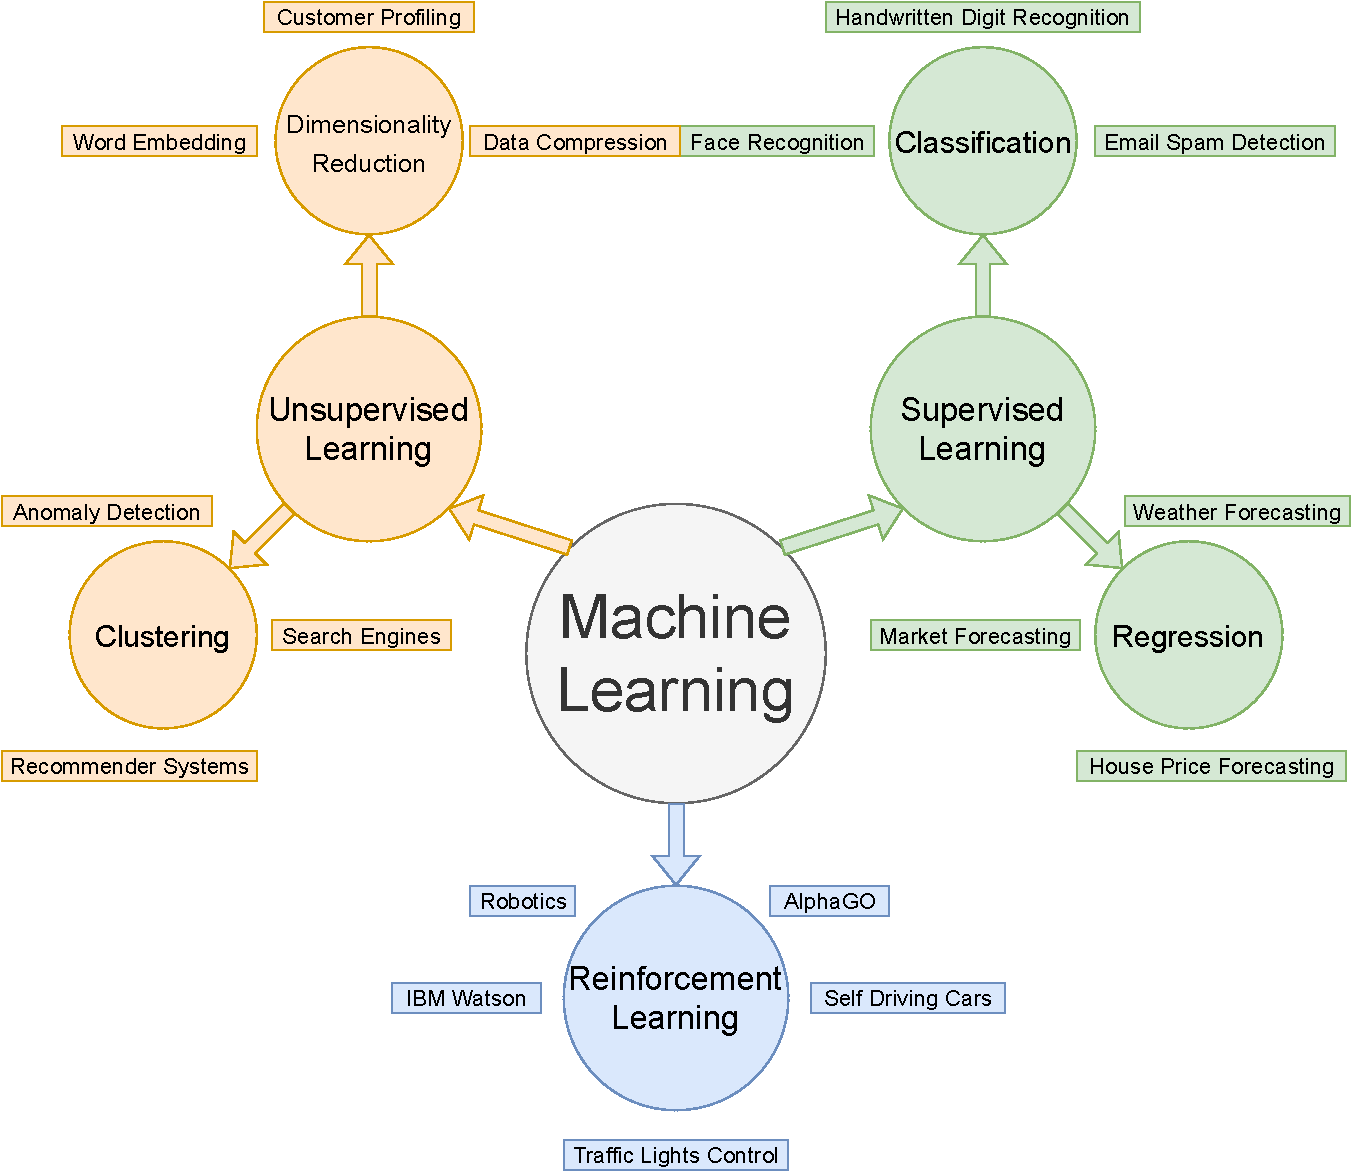
\includegraphics[width=\textwidth]{mlbasics/mlparadigms.pdf}
  \caption[Machine learning main paradigms]{Some applications of the three main machine learning paradigms.}
  \label{fig:paradigms}
\end{figure}


\section{Supervised learning}
\label{sec:sl}
As its name suggests, the learning is done in a supervised manner, like a teacher will supervise his students. To be used, supervised learning algorithms need a set of data, called the \emph{training dataset}, i.e. the data from which the underlying function is learned. The training data is composed of tuples of two elements. The first element is an input/entry element, and the second is the known answer corresponding to the input element, called the \emph{label}\footnote{\url{https://deepai.org/machine-learning-glossary-and-terms/supervised-learning}}. The goal of supervised learning algorithms is to find the relation between the input data and their corresponding labels, or in mathematical terms, to find the underlying function $f: X \to Y$ such as:
\begin{equation}
  f(x) = y
\end{equation}
where $x \in X$ is an element of the input space $X$ and $y \in Y$ its corresponding label in the decision space $Y$. The so called training dataset $D$ is then a set of tuples containing an element $x_i$ of the input space with its corresponding label $y_i$, so mathematically $D = \{(x_i, y_i), i \in \{1, ..., n\}\}$. To best approximate $f$, i.e. to learn from the training data, the algorithm starts with a solution $h_1$, and constructs a prediction $\hat{y}$ based on the input $x$, such as:
\begin{equation}
  h_1(x) = \hat{y}
\end{equation}
Then, it compares the true label $y$ with the prediction $\hat{y}$. Depending on this comparison, the algorithm modifies a bit the solution $h_1$ into the improved solution $h_2$. This process is iterated, and the solution is improved and will approximate better and better the true underlying function $f$. The quality of the prediction of the model is verified by using \emph{loss functions}.

\subsection{Loss functions}
A loss function estimates the cost or severity of predicting the actual prediction $h(x_i) = \hat{y}_i$ rather than the real value $y_i$. With that information, the algorithm knows if it is improving in a good direction, and have an idea how to minimze this loss. There are many loss functions that have different form, and that are more or less representative on specific applications. Given a training data point $(x_i, y_i)$ and a model $h$ to train, here are some often used loss function examples. Firstly, the \emph{squared error loss} is given by:
\begin{equation}
\label{eq:squaredloss}
  L(h(x_i), y_i) = (y_i - h(x_i))^2
\end{equation}
This is one of the simpliest and most used loss function for a regression problem. A small variation of this loss function that is often used is to add a factor $\frac{1}{2}$ to simplify computing the derivative. As second example loss function, the \emph{hinge loss} is used for binary classification, by penalizing the wrong prediction, but also the right ones that are not confident. It has the form:
\begin{equation}
  L(h(x_i), y_i) = \text{max} (0, 1 - y_i \cdot h(x_i))
\end{equation}
Finally, a similar loss function to the first loss function~\eqref{eq:squaredloss} is the \emph{absolute error loss}, given by:
\begin{equation}
  L(h(x_i), y_i) = |y_i - h(x_i)|
\end{equation}
This third loss function is more robust than the squared error because it is generally not affected by outliers. But on the other side, the squared error tends to adapt the model regarding the outliers. The loss function gives the information about how bad or good is one prediction. For an entire training dataset, the sum of the losses of all points in the dataset is required and will be more representative. This sum is called the \emph{empirical risk}, and will be used also further to tune neural networks. The empirical risk is given by:
\begin{equation}
  \hat{R}(h) = \sum^n_{i=1} L(h(x_i),y_i)
\end{equation}
The empirical risk can be averaged by a factor $\frac{1}{n}$ in certain cases, for example with the backpropagation algorithm (see further in Section~\ref{sec:backprop}).

A key point in the training phase is not to learn too much from the given data. Indeed, as stated in introduction of this chapter, the training data is only a subset of the real whole data. When the algorithm learns the available data too closely, it specializes on this precise data and is not able to predict well the future unseen data, resulting in a bad generalization. This phenomenon is called \emph{overfitting}.

Finally, supervised learning is mainly used for classification or regression problems, and is one of the most used paradigms in machine learning. A class of algorithm that are very strong with supervised learning are neural networks. In the following section, neural networks will be presented in detail.

\section{Neural Networks}
Nowadays, an extremely important concept that is used in machine learning is the \emph{neural network}. Neural networks are inspired by biological brains, that connect neurons with synapses. The concept of the natural neural network and the artificial neural network is to pass some information by connections. Neural networks are commonly trained using supervised learning. Figure~\ref{fig:neuron} shows the form of an artificial neuron, in comparison with biological neuron technical terms.
\begin{figure}[t!]
  \centering
  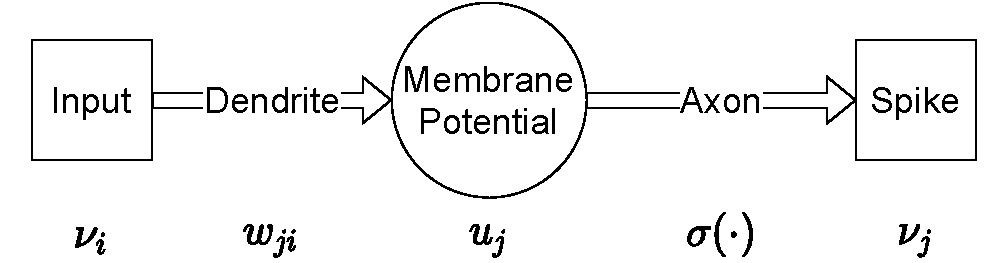
\includegraphics[width=\textwidth]{mlbasics/neuron.pdf}
  \caption[Schema of an artificial neuron]{Schema showing how an artificial neuron works. The input $\nu_i$ of the neuron is first weighted by some weight $w_{ji}$ that represents the connection beetween $i$ and $j$. The result is the membrane potential $u_j$, that is finally activated by an activation function $\sigma(\cdot)$. The output of the neuron is given by $\nu_j$.}
  \label{fig:neuron}
\end{figure}

An artifical neural network is composed of many neurons distributed in \emph{layers}. A neural network can have a variable number of layers depending on the task. Each layer is more or less connected to each other by neurons. Different shape of connections make different type of neural network. In each layer, there is one or several neurons. Each neuron has one or more inputs, that are the output of the neurons of the previous layer, but only one output. The neuron will take its inputs, arrange them according learned weights, and activate using an \emph{activation function}, and finally give the output. Mathematically, this is represented by the following formulas:
\begin{align}
  \begin{split}
    u_j &= \sum^k_{i=1} w_{ji} \cdot \nu_i \\
    \nu_j &= \sigma(u_j)
  \end{split}
\end{align}
where $u_j$ is the membrane potential of the neuron, $\nu_i$ are the inputs of the previous layer, $w_{ji}$ the synaptic weight of the neuron of the connection $i$ to $j$, and $\nu_j$ the output of the neuron, after activation with $\sigma(\cdot)$. There are several activation functions that can be used, for example the \emph{logistic} function:
\begin{equation}
  \sigma(x) = \frac{1}{1 + e^{-x}}
\end{equation}
As second example, the \emph{hyperbolic tangent}:
\begin{equation}
  \sigma(x) = \text{tanh}(x) = \frac{2}{1 + e^{-2x}} - 1
\end{equation}
Or the \emph{rectified linear unit} (ReLU) function:
\begin{equation}
  \label{eq:relu}
  \sigma(x) = \begin{cases}
    0 & \text{if } x < 0 \\
    x & \text{if } x \geq 0
  \end{cases}
\end{equation}
And at last example, the \emph{exponential linear unit} (ELU):
\begin{equation}
  \label{eq:elu}
  \sigma(x) = \begin{cases}
    \alpha (e^{x} - 1) & \text{if } x < 0 \\
    x & \text{if } x \geq 0
  \end{cases}
\end{equation}
These activation functions are again choosen depending on the task the neural network needs to do. For example, the logistic function will be more used for a binary classification task, as its output range is from 0 to 1, and can represent a probability. Compared to this, the hyperbolic tangent has the advantage to have an output range from -1 to 1. The two other examples, the ReLU and ELU are some of the most common choices in deep learning and convolutional networks. Both have their output range that goes towards infinity, but they differ in the lower bound. ReLU puts its negative values to zero immediately, whereas ELU will have a lower bound equal to $\alpha$. ELU has so the advantage to treat smoothly the negative values but at the cost to be slower to compute than the ReLU\footnote{\url{https://towardsdatascience.com/activation-functions-neural-networks-1cbd9f8d91d6}}.

The functioning of a neural network is the following. An input is given to the network, and it goes through several layers inside the network. At each layer, more or less outputs go out, and enter the next layer. At the other side of the network, in the last layer, the output of the network goes out, and is the final output, given the very first input. The output can have a very different form regarding the task that has to be achieved. For example, if a neural network is constructed to recognize if there is a cat in an image, then the input will be an image, and the output will be a binary output, with probabilities of true (there is a cat) or false (there is no cat).

Figure~\ref{fig:neuralnetwork} represents a neural network with two inputs $x_1$ and $x_2$, one hidden layer of two neurons $n_1$ and $n_2$, and one output layer of one neuron $n_3$. The weights are represented as $w_{ji}$. The computations inside the network go as follows. First, the weights are putting in a weight matrix, one matrix between each layer. The matrix between the inputs and the hidden layer is $W_{in}$, as the matrix between the hidden layer and the ouput layer is $W_{hid}$. Then, the inputs are stored in a vector $x$, the intermediate results are in the vector $n_{hid}$ and the output in $n_{out}$. The activation function in each neuron is $\sigma(\cdot)$. These definitions are given by:
\begin{align}
  \begin{split}
    W_{in} = \begin{pmatrix}
      w_{11} && w_{12}\\
      w_{21} && w_{22}
    \end{pmatrix}, \hspace{0.8cm}
    W_{hid} = \begin{pmatrix}
      w_{31} && w_{32}
    \end{pmatrix} \\
    x = \begin{pmatrix}
      x_1\\ x_2
    \end{pmatrix}, \hspace{0.8cm}
    n_{hid} = \begin{pmatrix}
      n_1\\ n_2
    \end{pmatrix}, \hspace{0.8cm}
    n_{out} = \begin{pmatrix}
      n_3
    \end{pmatrix}
  \end{split}
\end{align}
With the help of these definitions, the formulas to compute the intermediate results can be written using matrices multiplication from linear algebra:
\begin{align}
  \begin{split}
    n_{hid} &= \sigma(W_{in}x) = \begin{pmatrix}
      \sigma(w_{11} x_1 + w_{12} x_2)
      \sigma(w_{21} x_1 + w_{22} x_2)
    \end{pmatrix} \\
    n_{out} &= \sigma(W_{in} n_{hid}) = \begin{pmatrix}
      \sigma(w_{31} n_1 + w_{32} n_2)
    \end{pmatrix}
  \end{split}
\end{align}
And the full equation for the output of the example network can be written using the two equations above:
\begin{equation}
  \text{out} = n_3 = \sigma(w_{31} \sigma(w_{11} x_1 + w_{12} x_2) + w_{32} \sigma(w_{21} x_1 + w_{22} x_2))
\end{equation}

\begin{figure}[t!]
  \centering
  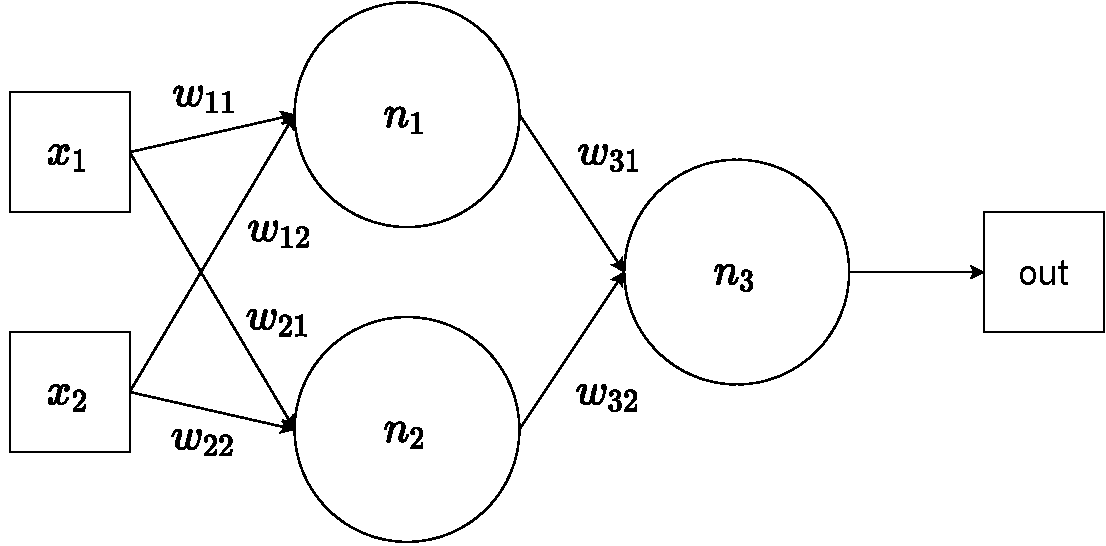
\includegraphics[width=\textwidth]{mlbasics/neuralnetwork.pdf}
  \caption[Neural network example]{Schema representing an example neural network. It contains one hidden layer of two neurons $n_1$ and $n_2$, and one output layer of one neuron $n_3$. $x_1$ and $x_2$ are the two inputs of the network, whereas the neuron $n_3$ gives the output of the network. The $w_{ji}$ are the six weights.}
  \label{fig:neuralnetwork}
\end{figure}

Mathematically speaking, a neural network is an universal function approximator. That means that a neural network can approximate any function from a theoretical perspective. In that way, neural networks can be used for quite any applications, given a network large enough. Neural networks are parametrized by their structure, i.e. how the layers are disposed, their activation functions and their weights. Different values for the weights can lead to very different outputs, thus the weights need to be well tuned. To give values to the weights in an optimal manner, a well-known algorithm is used: the \emph{backpropagation}. This is the main algorithm to train the network and to tune its weights, in the way to do a specific application.

\section{Backpropagation}
\label{sec:backprop}
As stated in Section~\ref{sec:mloverview}, the backpropagation was invented in the end of the 1980's, by simultaneous works of different researchers. The backpropagation algorithm is used with neural networks, and will adapt or optimize the weights of the network. Backpropagation is composed of two phases. The first one is called the \emph{forward pass}, when the inputs are propagating from the front of the network to the back, i.e. the network makes a prediction. Then, the prediction is compared to the ground truth label, and the error is computed with a loss function. In the second phase called the \emph{backward pass}, the error is propagating from the back of the network to the front. For each layer, the derivative of the error is computed. These derivatives help to know which weights contributed to the error, and help adapting them in a focused manner.

For a network, the backpropagation algorithm computes the error as the risk over all points of the dataset. The error depends on the weights set $w$ of the network. Indeed, different weights lead to different predictions, thus different errors. Let the error $E(w)$ of the network be:
\begin{equation}
  \label{eq:generalerrfun}
  E(w) = \frac{1}{|S|}\sum_{i \in S} L(f_w(x_i), y_i)
\end{equation}
with $f_w(\cdot)$ the function representing the network with specific weights $w$, $L(\cdot, \cdot)$ a choosen loss function, and $S$ a sample of the training data. This sample $S$ can be different regarding the type of training that is made. For example, $S$ can be the whole training dataset and the training is called to be in batch mode. In contrast, the sample can be choosen to be $|S| = 1$, that is called in online mode. But the most common way to train nowadays is the so called mini batches, by choosing $|S| \ll n$, that is in a small subset at each step of the learning. In general for backpropagation, the loss function used is the squared loss~\eqref{eq:squaredloss} with a $\frac{1}{2}$ factor. The error function~\eqref{eq:generalerrfun} for backpropagation will then be:
\begin{equation}
  \label{eq:backerrorfunction}
  E(w) = \frac{1}{2|S|}\sum_{i \in S} (f_w(x_i) - y_i)^2
\end{equation}

Note that in the following paragraphs and formulas, the symbols in superscript within parenthesis will represent the number of the current layer, as the symbols in subscript will represent the number of the neuron it refers. As example, the notation $\nu^{(l)}_n$ will refer to the output after activation of the $n$-th neuron of the layer $l$.

The goal of the backpropagation is to minimize the error function~\eqref{eq:backerrorfunction} of the network, to make the network as strong as possible in its predictions. To do that, weights must be tuned and adapted to make the best results. To know in which direction the weights must be changed regarding the error, backpropagation uses \emph{gradient descent}. This method iteratively finds a local mimimum or maximum of a differentiable function. In this method, the gradient of the increasing error is $\nabla_w E(w)$, and so the direction of the decreasing error will be in the opposite direction of the gradient, i.e in $-\nabla_w E(w)$ direction. A learning rule for a single weight can then be derived as:
\begin{equation}
  w^{(k)}_{ji} \gets w^{(k)}_{ji} - \eta \cdot \nabla_w E(w)
\end{equation}
where $\eta$ is called the learning rate. This rule shows that the weights are updated regarding the most decreasing error direction. As the error function $E(w)$ is differentiable with respect to the weights $w$, gradient descent can be applied and that is what backpropagation does. Mathematically\footnote{\url{https://brilliant.org/wiki/backpropagation/}}, the error gradient with the weight for neuron $j$ in layer $k$ connected to incoming neuron $i$ of previous layer is defined as:
\begin{equation}
  \nabla_w E(w) = \frac{\partial E}{\partial w^{(k)}_{ji}}
\end{equation}
Remember that in Figure~\ref{fig:neuron}, $u_j^{(k)}$ was denoted to be the membrane potential of neuron $j$ in the layer $k$, that is the value before going in the activation function. Let $n^{(k)}$ defines the number of neuron in the layer $k$, $u_j^{(k)}$ is computed by the sum:
\begin{equation}
  \label{eq:layeroutput}
  u_j^{(k)} = \sum^{n^{(k-1)}}_{m=1} w^{(k)}_{jm} \nu^{(k-1)}_m
\end{equation}
The partial derivative of the error with respect to one weight is computed using the chain rule, and is then given by:
\begin{equation}
  \label{eq:errorgradient}
  \frac{\partial E}{\partial w^{(k)}_{ji}} = \frac{\partial E}{\partial u_j^{(k)}} \frac{\partial u_j^{(k)}}{\partial w^{(k)}_{ji}}
\end{equation}
The first term of~\eqref{eq:errorgradient} is in general called the backpropagated error, and is written as:
\begin{equation}
  \label{eq:errorterm}
  \delta_j^{(k)} = \frac{\partial E}{\partial u_j^{(k)}}
\end{equation}
Whereas the second term is calculated to be $\nu_i^{(k-1)}$ the output after the activation of the neuron $i$ in the layer $k-1$, i.e. the previous layer:
\begin{equation}
  \frac{\partial u_j^{(k)}}{\partial w^{(k)}_{ji}} = \frac{\partial}{\partial w^{(k)}_{ji}} \left( \sum^{n^{(k-1)}}_{m=1} w^{(k)}_{jm} \nu^{(k-1)}_m \right) = \nu_i^{(k-1)}
\end{equation}
In summary, the derivative of the error~\eqref{eq:errorgradient} regarding a weight can be written in the compact form:
\begin{equation}
  \label{eq:errorcompact}
  \frac{\partial E}{\partial w^{(k)}_{ji}} = \delta_j^{(k)} \nu_i^{(k-1)}
\end{equation}

On one hand, for the output layer $l$, i.e. the last layer of the network, \eqref{eq:errorcompact} will depend directly on the label $y$ and the prediction $f_w(y)$. By applying the chain rule and using the derivative of~\eqref{eq:backerrorfunction}, the derivative of the error that is~\eqref{eq:errorcompact} will become:
\begin{equation}
  \frac{\partial E}{\partial w^{(l)}_{ji}} = \delta_j^{(l)} \nu_i^{(l-1)} = (f_w(y) - y) \cdot \sigma'\left( \sum^{n^{(k-1)}}_{m=1} w^{(l)}_{jm} \nu^{(l-1)}_m \right) \cdot \nu_i^{(l-1)}
\end{equation}
On the other hand, for a hidden layer $k$, the error term~\eqref{eq:errorterm} is first computed by again using the chain rule:
\begin{equation}
  \delta^{(k)}_j = \frac{\partial E}{\partial u_j^{(k)}} = \sum^{n^{(k+1)}}_{m=1} \frac{\partial E}{\partial u_m^{(k+1)}} \frac{\partial u_m^{(k+1)}}{u_j^{(k)}}
\end{equation}
But the first term in this sum represents also an error term~\eqref{eq:errorterm}. By using the definition and derivative of~\eqref{eq:layeroutput}, the error term for hidden layers will become:
\begin{equation}
  \label{eq:hidlayerror}
  \delta^{(k)}_j = \sum^{n^{(k+1)}}_{m=1} \delta^{(k+1)}_m \cdot w^{(k+1)}_{jm} \cdot \sigma'(u^{(k)}_j)
\end{equation}
Finally, by taking the result of~\eqref{eq:hidlayerror}, the derivative of the error~\eqref{eq:errorcompact} for hidden layers will be:
\begin{equation}
  \frac{\partial E}{\partial w^{(k)}_{ji}} = \sigma'(u^{(k)}_j) \cdot \nu_i^{(k-1)} \cdot \sum^{n^{(k+1)}}_{m=1} \delta^{(k+1)}_m \cdot w^{(k+1)}_{jm}
\end{equation}
This last equation shows that the error at layer $k$ is also depending on the error at layer $k+1$, that means that the computations of these errors must be done backwards. That is where the backpropagation algorithm takes its name. Figure~\ref{fig:backprop} shows the two steps of the backpropagation: the forward pass where the prediction is made, and the backward pass where the errors are computed.
\begin{figure}[t!]
  \centering
  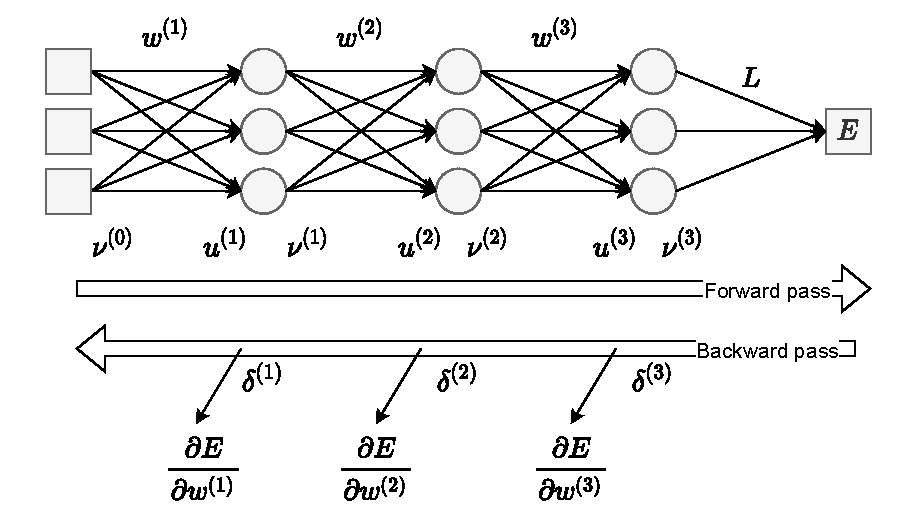
\includegraphics[width=\textwidth]{mlbasics/backprop.pdf}
  \caption[Backpropagation algorithm schema]{Schema representing the backpropagation algorithm steps. First, the forward pass is done, where the input $\nu^{(0)}$ go through the network, generating an output prediction. This prediction $\nu^{(3)}$ is compared with the actual target label, and the error $E$ is computed using the loss $L$. During the backward pass, the errors $\delta^{(i)}$ are computed, and used in the calculation of the partial derivatives. This derivatives help to adjust the weights $w^{(i)}$ of the neural network.}
  \label{fig:backprop}
\end{figure}

\section{Deep learning}
\label{sec:deeplearning}
In the recent years, some of the best results of the field come from \emph{deep learning}. Deep learning is a learning technique that uses a neural network containing many layers. That makes the network, as the name suggests, a deep network. Deep learning starts to appear in the 2010's. Before that time, it was not possible to develop deep learning. Main factors that have helped the development of deep learning were the multilayers neural networks, \emph{big data}, and the power of computations of the machines that are now enough strong to compute deep learning algorithms. The foundation of deep learning is contained in the work of \citet{goodfellow_deep_2016}, that was published in 2016.

Deep learning is used in many applications such as translators, image processing, natural language processing, and others. A major problem with deep learning however, is that the deep networks need a lot of data to be trained, which is not always easy to obtain. For example, in medical applications, the privacy of the patients data makes it difficult to collect enough data to use with deep learning. Indeed, personal information of the patients are sensible, and hence must be removed before giving public access to the data, as in the Cancer Imaging Archive.

\subsection{Convolutional neural networks}
From image classification to object detection, computer vision is used in different applications such as face recognition, autonomous cars or for military purpose. One of the most popular neural network model used for computer vision is the \emph{convolutional neural network} (CNN). One of the first CNN was when \citet{lecun_backpropagation_1989} used backpropagation to recognize handwritten zip codes. Convolutional neural networks take an image as input, and can do several tasks, such as classification, localization or segmentation (see Section~\ref{sec:tasks}).

The general structure of a convolutional neural network is composed of a first part called \emph{feature extractor} or feature learning part, that is a combination alternating \emph{convolutional layers} and \emph{pooling layers}. The second part is one or more fully connected layers that is a \emph{decision maker}. Figure~\ref{fig:cnn} shows the general architecture of a CNN.

\begin{figure}[t]
  \centering
  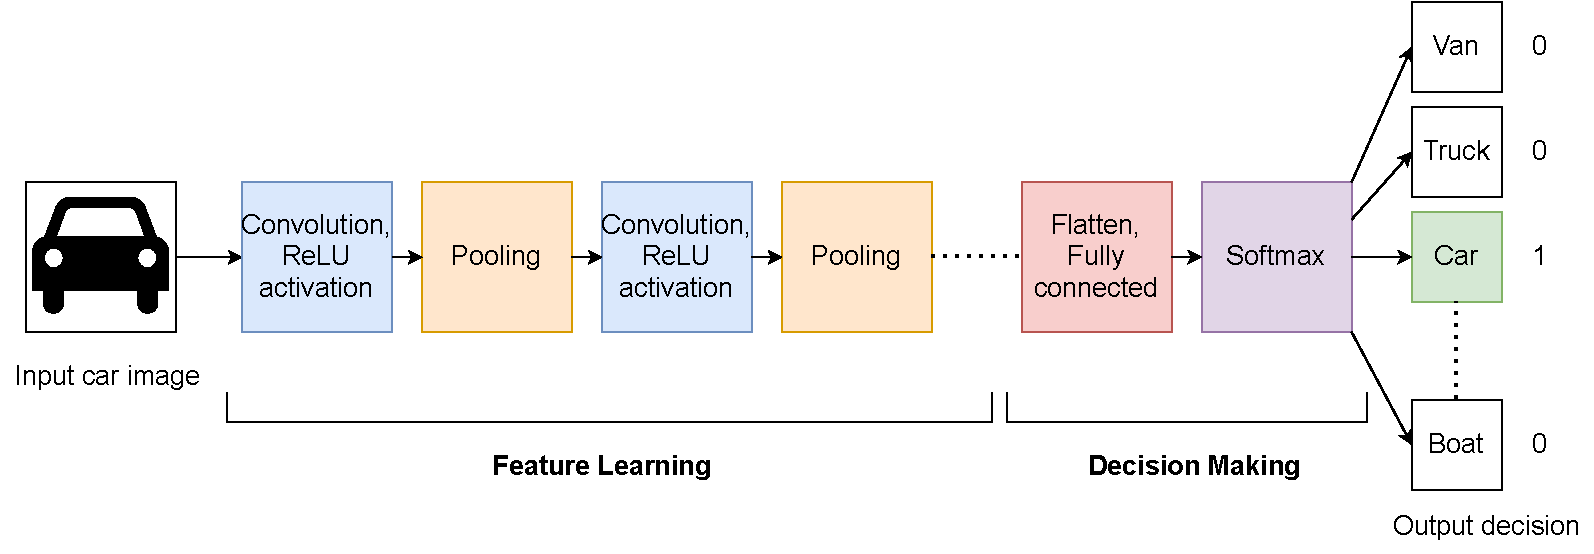
\includegraphics[width=0.96\textwidth]{mlbasics/cnn.pdf}
  \caption[Architecture of a convolutional neural network]{General architecture of a convolutional neural network. The first part represents a feature extractor, that analyzes the input image by several convolutions and poolings to extract features. These features are fed to the second part, that is a decision maker. In this example, the decision maker is a multi-class classifier that will output the probability that the image is a given vehicle, with the help of the last softmax layer that outputs a vector of probability to be in a given class.}
  \label{fig:cnn}
\end{figure}

To extact features of an image, CNNs alternate convolutions and poolings. Convolution is a mathematical operation between two objects that indicates correlated features of these objects. In computer vision, the two objects used in a convolution are the input image itself and a \emph{kernel} or \emph{mask}. A kernel is a two dimensional matrix. The form and the values of the kernel will define the effect of the convolution when applied to the image. For example, kernels can detect ridges, vertical or horizontal lines, or sharp the image. To perform a convolution, a window (subarea of the image) containing the kernel values will slide over the image iteratively. At each step, a convolved feature is outputed. Convolutions are characterized by parameters such as the size of the kernel, the stride i.e. by how much the window is moved in a single iteration, and paddings that can add pixel in the border of the image. Depending on these parameters, the outputed convolved features can have the same size, or a reduced dimensionality compared to the input image. Figure~\ref{fig:convolution} shows 4 steps during a convolution, that applies an element-wise multiplication between the image and the kernel.

\begin{figure}[t]
  \centering
  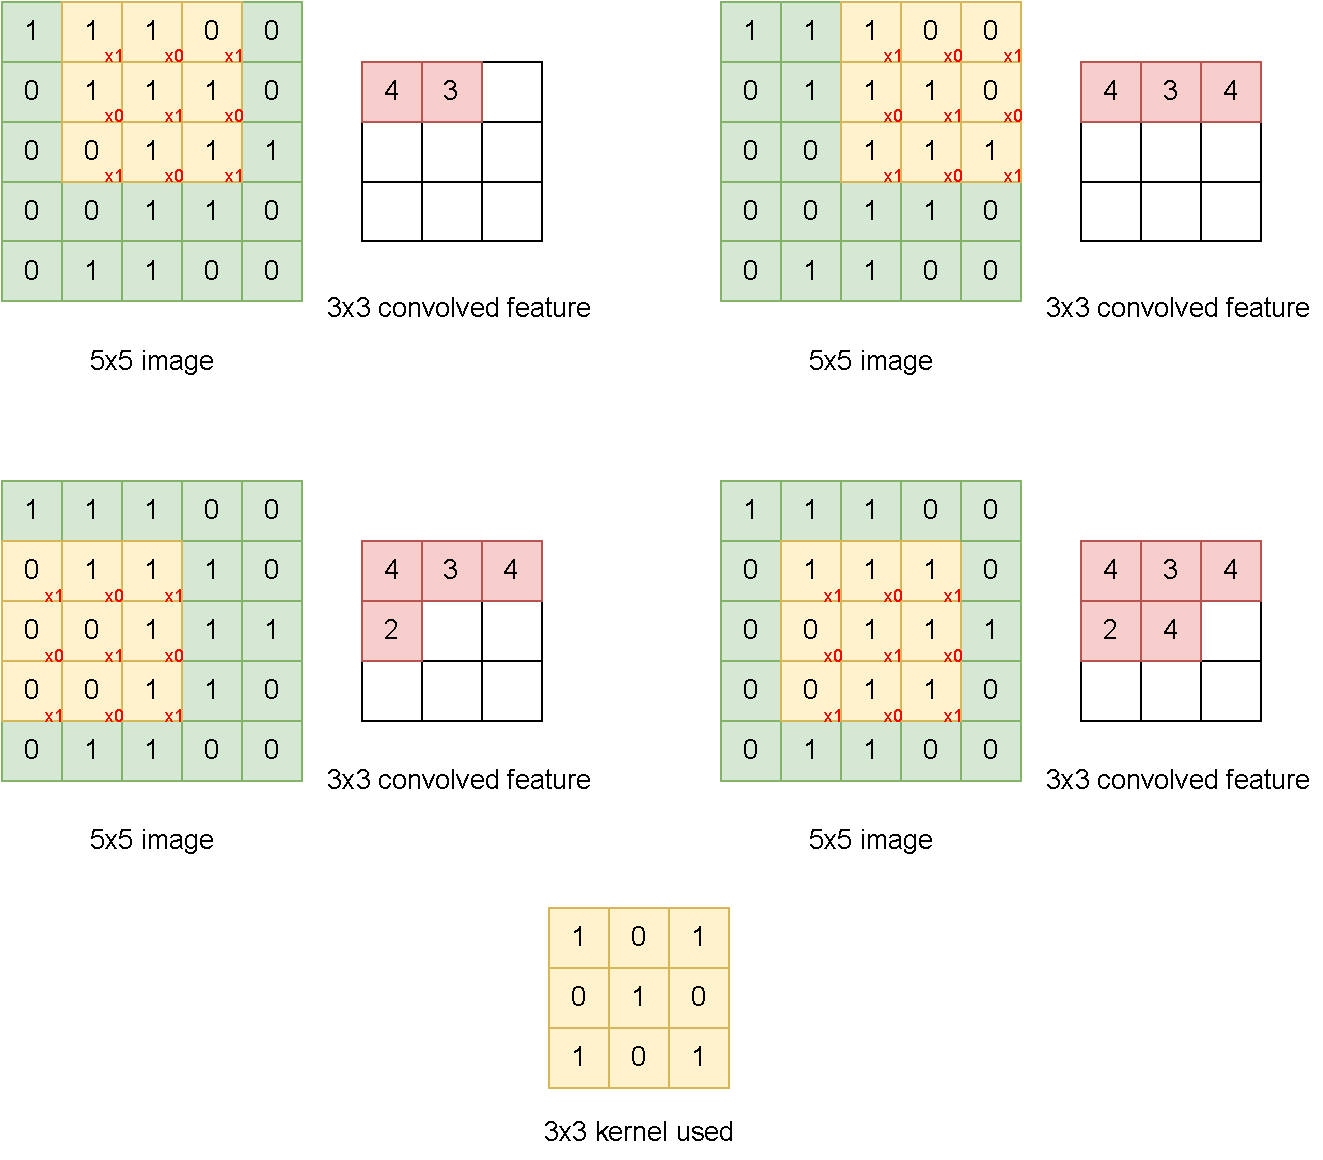
\includegraphics[width=\textwidth]{mlbasics/convolution.pdf}
  \caption[Convolution steps example]{Four example steps during a convolution. A 3x3 window (yellow) containing the kernel values is sliding on an 5x5 image (green) and contructs a 3x3 convolved feature result (red) by an element-wise multiplication.}
  \label{fig:convolution}
\end{figure}

After a convolution, a pooling is performed. The pooling will reduce the dimensionality of the image, and extract the most dominant features that are invariant under translation and rotation. The pooling also uses sliding windows over the convolved image, that will output a specific characteristic depending on the type of pooling. The two most used poolings are the \emph{max pooling}, which extracts the maximal value in the kernel, or the \emph{average pooling} that extracts the average value of all values in the kernel. In case of CNN, the max pooling is typically prefered. Figure~\ref{fig:pooling} shows how the max and average pooling are performed.

\begin{figure}[t!]
  \centering
  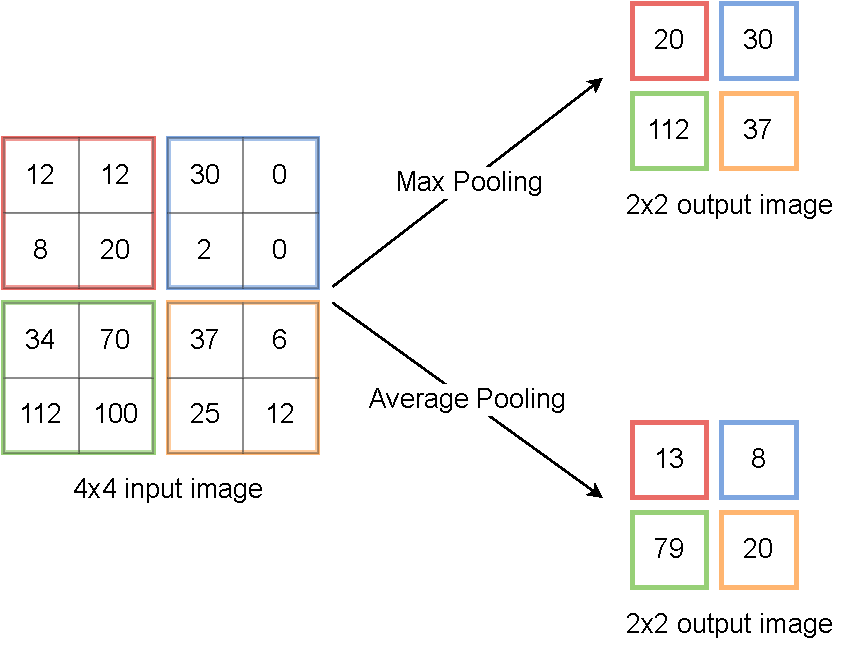
\includegraphics[width=0.62\textwidth]{mlbasics/pooling.pdf}
  \caption[Two of the main types of pooling]{Two of the main types of pooling. Here, a 2x2 kernel is used. The max pooling extracts the maximal value of the kernel, while the average pooling extracts the average of all values within the kernel.}
  \label{fig:pooling}
\end{figure}


\section{Computer aided diagnosis tasks}
\label{sec:tasks}
In the last decades with machine learning and artificial intelligence coming more and more popular and powerful, improvements have been made in the medical field too. With the possibility to use computers to analyze several types of images for many purpose, medical images can be analyzed as well. Techniques can help radiologists in their work, as a second opinion or to detect primary signs of cancer that humans can miss. These techniques are called \emph{Computer Aided Diagnosis} (CAD) systems~\cite{doi_computer-aided_2007}. With the development of deep learning, CAD systems become more and more precise and powerful, by using convolutional neural networks to analyze medical images and perform different tasks, such as classification, localization and segmentation.

\subsection{Classification}
Classification is the task to partition images depending on their characteristics (features). Classification can be binary, i.e. with only two classes, or multi-class. CAD systems can perform this task for example to classify images in a binary manner: The positive class regroups images containing one or more malignant tumors, while the negative class contains images having no malignant masses. The CNN of a CAD system can be trained using supervised learning, but it requires ground truth medical diagnosis. The medical images are the inputs of the network, while the medical diagnoses (true or false) are the labels. By feeding a significant amout of data, the CNN is train and can output a probability that an image contains a malignant tumor. The classification task performed by CAD systems can help radiologists to detect primarily stages of cancer.

\subsection{Localization}
Localization is the task to points the position of an object in an image. In the medical field, a precise location of a malignant tumor is required when doctors are ablating (removing) it. CAD systems can also perform localization: given a medical image in input, they can tell a position where they find a malignant tumor. When training in a supervised learning manner, CAD systems need images as inputs but also ground truth positions (as coordinates for example) of malignant tumors within the image as labels. Finally, an overlay can for example display the location of the tumor outputed by the CAD system.

\subsection{Segmentation}
\label{sec:cadsegtask}
In the medical field, \emph{segmentation} is the process to delimit or contour a specific body part. On one hand, CAD systems can segment organs: for example, \citet{litjens_evaluation_2014} analyzed the results of the 2012 \emph{Prostate MR Image Segmentation} (PROMISE12) challenge organized by the Medical Image Computing and Computer Assisted Intervention society (MICCAI)\footnote{\url{http://www.miccai.org/}}. The goal of this challenge was to develop CAD systems that can perform the segmentation of the prostate, given MRIs of the prostate as inputs. On the other hand, CAD systems can segment malignant tumors: for example, \citet{wang_transbts_2021} develop a CAD system capable of segmenting brain tumors. CAD systems can do segmentation in two or three dimensions. Like classification and localization, segmentation can also be trained with supervised learning. The inputs are the medical images, and the labels are the so called \emph{segmentation masks}. These masks are monochrome (binary) images that have the same size as the input image. Each pixel of the segmentation mask corresponds to a pixel in the medical image. If the pixel is black, the malignant tumor is not present in that position, while if the pixel is white, the tumor is present. Figure~\ref{fig:segmaskimg} illustrates an example of a medical image (input) in~\ref{fig:segmaskimg1} with its corresponding segmentation mask (label) in~\ref{fig:segmaskimg2}, and both are display in a same image in~\ref{fig:segmaskimg3}, where a malignant tumor is colored in red.

\begin{figure}[t!]
     \centering
     \begin{subfigure}[b]{0.32\textwidth}
         \centering
         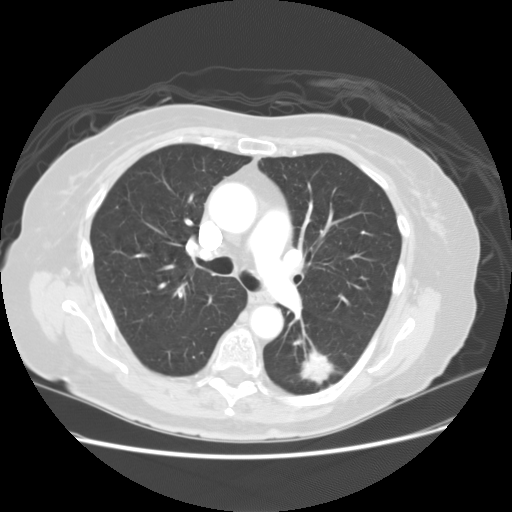
\includegraphics[width=\textwidth]{medicalcontext/medimg.png}
         \caption{CT scan of the lungs}
         \label{fig:segmaskimg1}
     \end{subfigure}
     \hfill
     \begin{subfigure}[b]{0.32\textwidth}
         \centering
         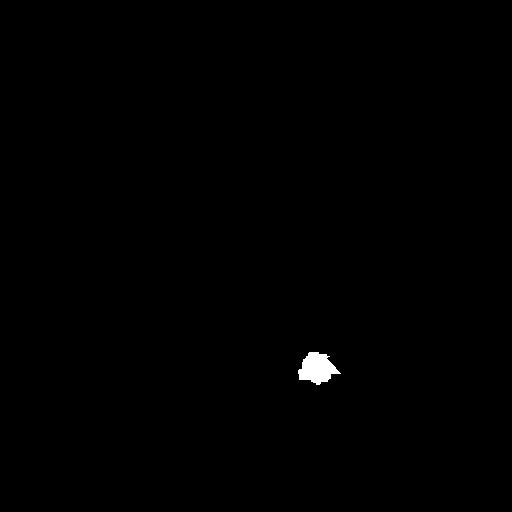
\includegraphics[width=\textwidth]{medicalcontext/segmask.png}
         \caption{Segmentation mask}
         \label{fig:segmaskimg2}
     \end{subfigure}
     \hfill
     \begin{subfigure}[b]{0.32\textwidth}
         \centering
         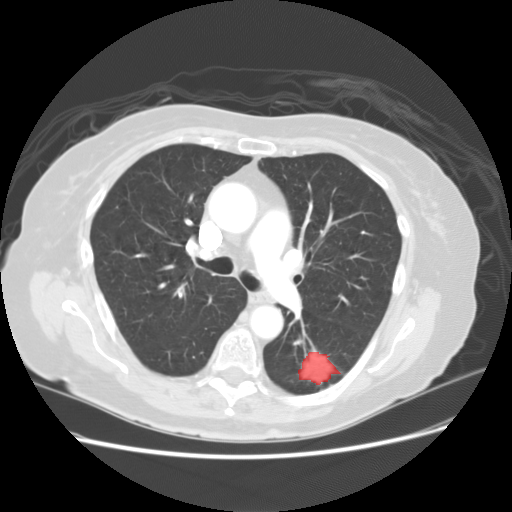
\includegraphics[width=\textwidth]{medicalcontext/imgmask.png}
         \caption{Tumor colored in red}
         \label{fig:segmaskimg3}
     \end{subfigure}
        \caption[Computed tomography scan of the lungs and its segmentation mask]{Example image of a computed tomography scan of the lungs and its segmentation mask from the LIDC-IDRI dataset~\cite{armato_data_2015}. The detected malignant tumor is colored in red in the right image.}
        \label{fig:segmaskimg}
\end{figure}


\section{Hydra framework}
As stated in the motivation of this work, the main goal of this project is to develop a CAD system with the collaboration of the H-FR. This CAD system can help the radiologists in their work. At this time, the Hydra project has been first trained to do tumor detection on the prostate, the lungs and the brain. The name Hydra comes from the shape of the network. It is composed of a body with many heads, like the mythical creature: The body is the feature extractor of the network, i.e. the part where the image is analyzed and convolved and is the same for all type of organs, because tumors share common characteristics. The multiple heads are a set of decision makers returning the probability or not to find a tumor. Each head is specialized for a precise organ. Currently, there is one head for the prostate, one for the lungs and one for the brain. When predicting a specific organ, the body of Hydra will be taken, and the head for the specific organ will be attached. In that way, the feature extraction is general enough to have a good intuition for the decision, and the decision maker is specialized enough to give the right decision for a specific organ. Figure~\ref{fig:hydra} shows the generic form of the Hydra CNN model.
\begin{figure}[t!]
  \centering
  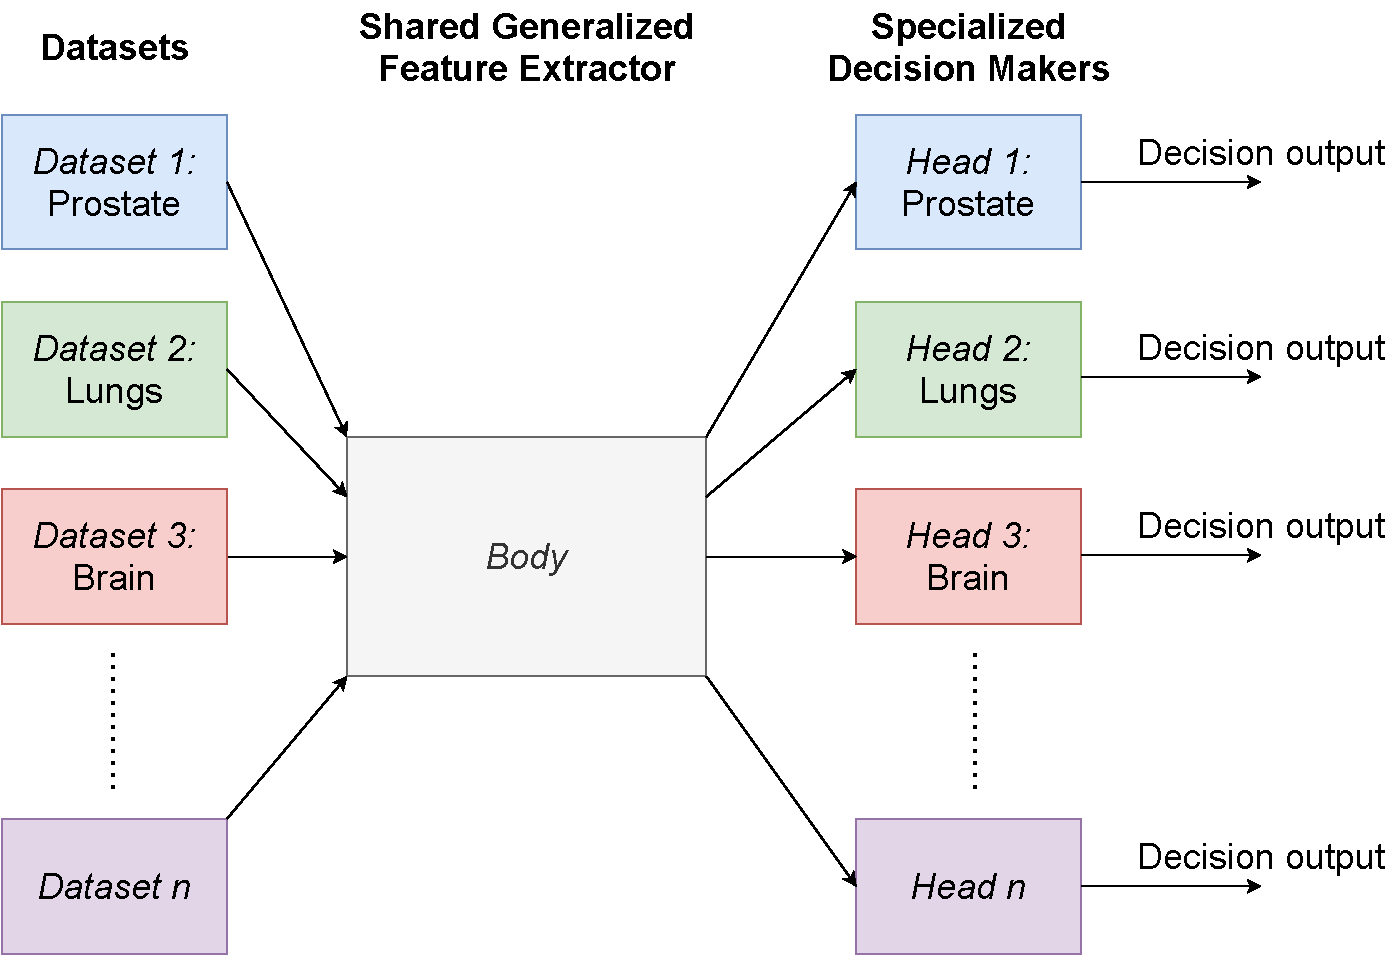
\includegraphics[width=\textwidth]{mlbasics/hydra.pdf}
  \caption[Hydra generic model]{Generic Hydra model. The body is a feature extractor and is common for all type of organs. The model has then many heads that are the decision makers, each head being specialized for one specific organ. The input dataset enters the network first in the shared feature extractor (the body), and goes to the specialized decision maker attached depending on the organ (the head). The decision goes out of the head.}
  \label{fig:hydra}
\end{figure}

This type of architecture avoids the problem of publicly available medical data scarcity stated in the Section~\ref{sec:deeplearning}. It has two advantages:

\vbox{
  \begin{enumerate}
    \item Hydra can learn features from tumors for any organs. Even if data is sparse for a new organ, Hydra uses what it has previously learned from other organs to extract features. In that way, the data used to train the feature extractor is augmented, by aggregating data of any organs. The feature extraction is then generalized.
    \item Each decision maker of Hydra is specialized only for one specific organ. Thus, the heads do not need a lot of data to be train. The scarsity of the data for an organ avoids the generalization of the heads, that could lead to incorrect predictions.
  \end{enumerate}}

The current convolutional neural network model used for Hydra is based on the VGG-16 model architecture~\cite{simonyan_very_2015}, where 16 is the number of layers in the model. The Hydra model contains 9 convolutional layers separated in 3 convolutional blocks of 5 layers each, and 4 fully connected layers at the end. The activation function used after the convolutions is the ELU~\eqref{eq:elu} (see Section~\ref{sec:sl}). Dropout layers are used to prevent overfitting, as training large neural network on relatively small training datasets could overfit the training dataset. To avoid that, dropout layers skip or ignore randomly some neuron's inputs and outputs during the process. This has the effect to preventing the neurons to co-adapt themselves too much during the training~\cite{srivastava_dropout_2014}. Figure~\ref{fig:hydralayers} shows the current full model Hydra with its separated blocks.
\begin{figure}[t!]
  \centering
  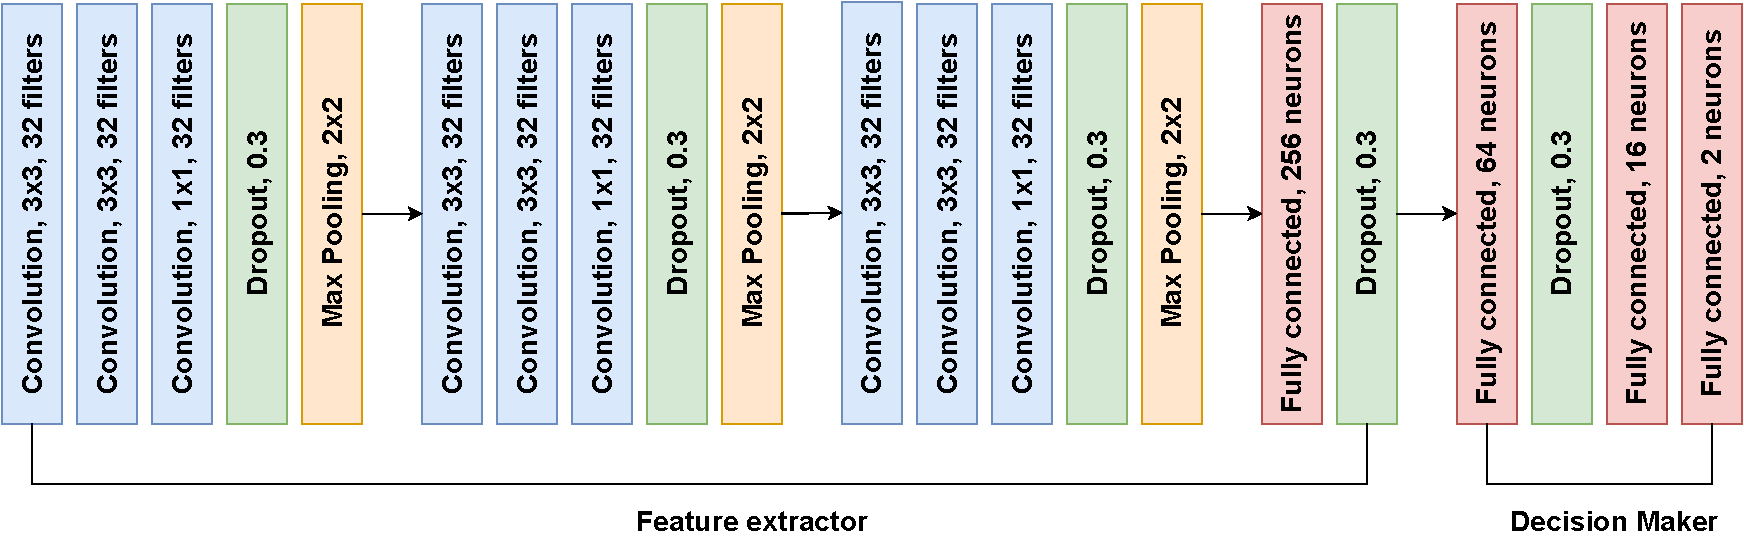
\includegraphics[width=\textwidth]{mlbasics/hydralayers.pdf}
  \caption[Hydra layers]{Full Hydra model, with its layers. The feature extractor is composed of 3 blocks of convolutions ending by a dropout and a max pooling layer. The decision maker is a block of fully connected layers.}
  \label{fig:hydralayers}
\end{figure}

% !TEX root = ../main.tex

\chapter{Datasets}
\label{ch:datasets}
This Chapter presents the three datasets that have been choosen to be part of this work. The first section, after a small introduction, explains how the choice of these datasets was made. Then, the types of medical images that are used in this work will be described. These types are ones of the most common used. At the end of the second section, a little detour is taken to present the DICOM standard, which is a common standard for medical imaging. Finally in the last section, the three datasets will be presented.


\section{Introduction and choices}
Deep learning models require a lot of data to be efficient (see Section~\ref{sec:deeplearning}). However, in research of deep learning methods in the medical field, data is often scarce. Indeed, lack of publicly available medical data is an issue because of the personal and sensible data of the patients. The data needs to be anonymized before publishing. Today, there exist such publicly available data, provided by the following ressource: the Cancer Imaging Archive (TCIA)~\cite{clark_cancer_2013} is funded by the National Cancer Institute (United States). The data is separated in collections, that have a common disease, the same medical images type (see Section~\ref{sec:medimtype}) or is at the base of a common research goal.

The first part of this work was to choose different datasets to preprocess. Different conferences, like the Medical Image Computing and Computer Assisted Intervention society (MICCAI)\footnote{\url{http://www.miccai.org/}}, the Medical Imaging with Deep Learning (MIDL)\footnote{\url{https://2021.midl.io/}} or the Machine Learning for Healthcare Conference (MLHC)\footnote{\url{https://www.mlforhc.org}} offer many publications in the scope of this work. About 25 publications coming from these conferences were read in detail, but only 5 were retained~\cite{wang_transbts_2021, xie_transferable_2017, ding_accurate_2017, andrearczyk_automatic_2020, wang_residual_2021}. The available datasets of these 5 publications went on a common list. Finally, the work can start with three new datasets choosen from this list. Two of them come directly from TCIA.


\section{Types of medical images}
\label{sec:medimtype}
Depending on the body part to look at, a different type of image or scan can be used. There exist many types of medical images, depending on the hardware, the technology used or the parameters for a same setup. The medical images types are sometimes called the \emph{modality} of the image. Modalities used in this work are:

\vbox{
  \begin{itemize}
    \item Magnetic resonance image (MRI)
    \item Computed tomography (CT) scan
    \item Positron emission tomography (PET) scan
    \item Ultrasound (US) image
  \end{itemize}}
These four modalities will be explained in detail in the following paragraphs. While CT, PET scans and US images come in the datasets presented in this work, the MRI modality comes from previous datasets preprocessed for the \emph{Hydra} framework in the work of~\citet{clement_prostate_2020}.

\subsection{Magnetic resonance image}
The first modality, the \emph{Magnetic resonance image}, produces three-dimensional images from the body, as a stack of 2D images. It uses a strong magnetic field, that will force the protons in the body to align with the field. With a magnetic field that has a frequency dependance, protons will align and dealign as the time passes. This motion of the protons and the energy released during the process is then captured by some sensors, that produce the image. MRI is more often used for soft tissues like muscles, ligments or tendons. For example, MRI is used for the knees, the shoulders or even the brain. To get the image, patients lie on a bed that goes inside a MRI scanner, that has the shape of a closed tunnel, and they stay fixed during the process~\cite{national_institute_of_biomedical_imaging_and_bioengineering_magnetic_nodate}. Figure~\ref{fig:mriprostate} shows a MRI of the prostate.

\subsection{Computed tomography scan}
The second type is the \emph{computed tomography scan}. These scans produce two-dimensional images that can then be stacked to form a full-body image, as for MRI. CT scans use X-rays, that are emitted and go through the body, and are then captured by detectors on the other side. A 2D image is then constructed. CT scans can better see hard tissues, like bones. It can then be used to see bones fractures, but also to image the lungs or the brain. To construct the image, patients lie on a bed that moves slowly through a scanner that has a ring shape. The scanner will emit the X-rays as the patient goes through~\cite{national_institute_of_biomedical_imaging_and_bioengineering_computed_nodate}. Figure~\ref{fig:ctlung} shows a CT scan of the lungs.

\subsection{Positron emission tomography scan}
The third type mentionned is the \emph{positron emission tomography scan}. While the two previous types were non-invasive techniques, the PET is invasive. The patient receives first an intravenous injection of a safe radioactive substance, called the \emph{radiotracer}. The radiotracer is absorbed by the body cells: cells that are diseased will absorb more radiotracer than the healthy ones. This is because the radiotracer accrues in cells that need a lot of glucose. As tumor cells need a significant amount of glucose, it is well absorbed by tumors. By going through a PET scanner, detectors can see which parts have absorbed more of the radiotracer, and can construct 2D images that will be stacked to form a full body three-dimensional image~\cite{cleveland_clinic_pet_nodate}. Figure~\ref{fig:petbrain} shows a PET scan of the brain.

\subsection{Ultrasound image}
Finally, the last type listed above is the \emph{ultrasound images}. This is also a non-invasive technique that uses ultrasound waves emitted from a device named transducer, that is directly touching the skin of the patient. The transducer first projects sound waves within the body, which travel and are then reflected by the different body parts. The transducer listens to the reflected waves, and by measuring the amplitude of the waves and the time they take to reflect, the transducer can compute a 2D image of the tissues and organs. The ultrasound image is then produced in realtime, and can capture the motion of the body parts. This type of image is widely used for several echography, or for breast imaging for example~\cite{national_institute_of_biomedical_imaging_and_bioengineering_ultrasound_nodate}. Figure~\ref{fig:usbreast} shows an ultrasound image of the breast (mammography).

\begin{figure}[t!]
     \centering
     \begin{subfigure}[t]{0.49\textwidth}
        \centering
        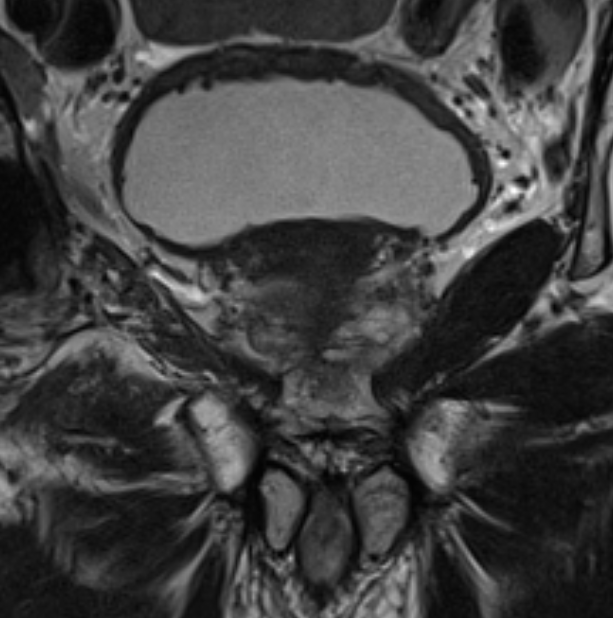
\includegraphics[height=0.25\textheight]{medicalcontext/mriprostate.png}
        \caption[Prostate magnetic resonance image]{Example of a magnetic resonance image of the prostate. This image comes from the PROSTATEx dataset~\cite{armato_prostatex_2018} and has been cropped from the original image.}
        \label{fig:mriprostate}
     \end{subfigure}
     \hfill
     \begin{subfigure}[t]{0.49\textwidth}
        \centering
        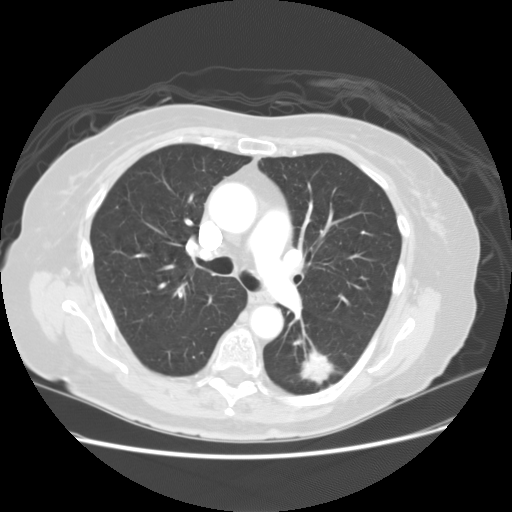
\includegraphics[height=0.25\textheight]{medicalcontext/medimg.png}
        \caption[Lungs computed tomography scan]{Example of a computed tomography scan of the lungs, taken from the LIDC-IDRI dataset~\cite{armato_data_2015}. At the bottom right of the image, a cancerous tumor can be seen, with its typical spider-web-shape.}
        \label{fig:ctlung}
     \end{subfigure}
     \\
     \begin{subfigure}[t]{0.49\textwidth}
        \centering
        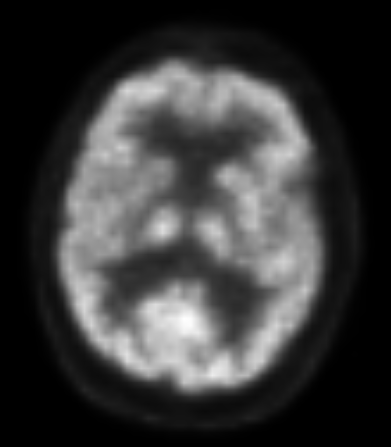
\includegraphics[height=0.25\textheight]{medicalcontext/petbrain.png}
        \caption[Positron emission tomography scan of the brain]{Example of a positron emission tomography scan of the brain from the HNPC dataset~\cite{vallieres_data_2017}.}
        \label{fig:petbrain}
     \end{subfigure}
     \hfill
     \begin{subfigure}[t]{0.49\textwidth}
        \centering
        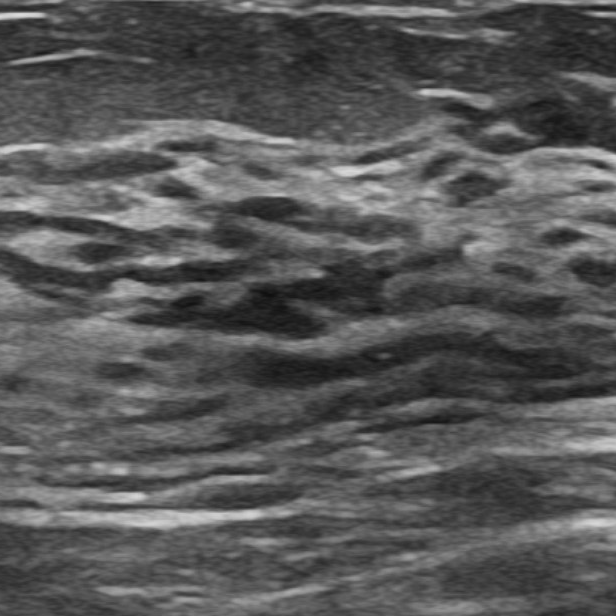
\includegraphics[height=0.25\textheight]{medicalcontext/usbreast.png}
        \caption[Breast ultrasound]{Example of an ultrasound image of the breast, taken from the BUSI dataset~\cite{al-dhabyani_dataset_2020}. This image has been cropped from the original image, to focus on the cancerous tumor.}
        \label{fig:usbreast}
     \end{subfigure}
        \caption[Four different medical images modalities]{Example figure that shows four different modalities of medical images.}
        \label{fig:segmaskimg}
\end{figure}


\section{DICOM standard}
\label{sec:dicom}
Different types of medical images need different hardware, scanners but also the screens on which the image is displayed, or the sensors. All this hardware setup will lead to compatibility problems. Indeed, hospitals around the world have not the exact same hardware to display or create the medical images. When patients go from one hospital to another, images could be displayed differently. To solve this problem, a standardization for medical image is introduced as the \emph{Digital Imaging and Communications in Medicine} (DICOM) standard for medical images and their information. Born in 1993 under the collaboration of the American College of Radiology (ACR) and the National Electrical Manufacturers Association (NEMA), the DICOM standard has revolutionized the medical world, both for doctors and patients. It has enabled advanced medical imaging system, and is one of the most deployed healthcare messaging system. DICOM is the \texttt{ISO~12052:2017} standard~\cite{mildenberger_introduction_2002}.

DICOM files can be recognized by their \texttt{.dcm} file extension. The structure of a \mbox{DICOM} file can be represented as a dictionary structure, each entry being a \mbox{key-value} pair. Keys are called \emph{DICOM tags} and are tuples of two hexadecimal numbers, uniquely identified, which correspond to a certain value. A tool that explains and describes all DICOM tags of all type of images is available at the DICOM standard browser\footnote{\url{https://dicom.innolitics.com/ciods}}. These hundred of different tags contain all medical information: from the patient information, to the size of the image, to the type of image, to some numeric identifiers, to settings of the scanner who takes the image. Each DICOM file contains all these tags but also one or more 2D images (slices), stored in a specific DICOM tag, named \texttt{Pixel Data}. Figure~\ref{fig:dicom} shows an example of DICOM tags available in a CT scan.

To solve the compatibility problems mentioned above, DICOM provides some information in its tags. For example, it provides slope and intercept values to rescale the image (tags \texttt{(0028,1052)} and \texttt{(0028,1053)}). Additional information like the pixel spacing (tag \texttt{(0028,0030)}) or bits allocated (tag \texttt{(0028,0100)}) are also useful to normalize images from a dataset. Section \ref{sec:imgconversion} shows more technical details to convert medical images.

\begin{figure}[t!]
  \centering
  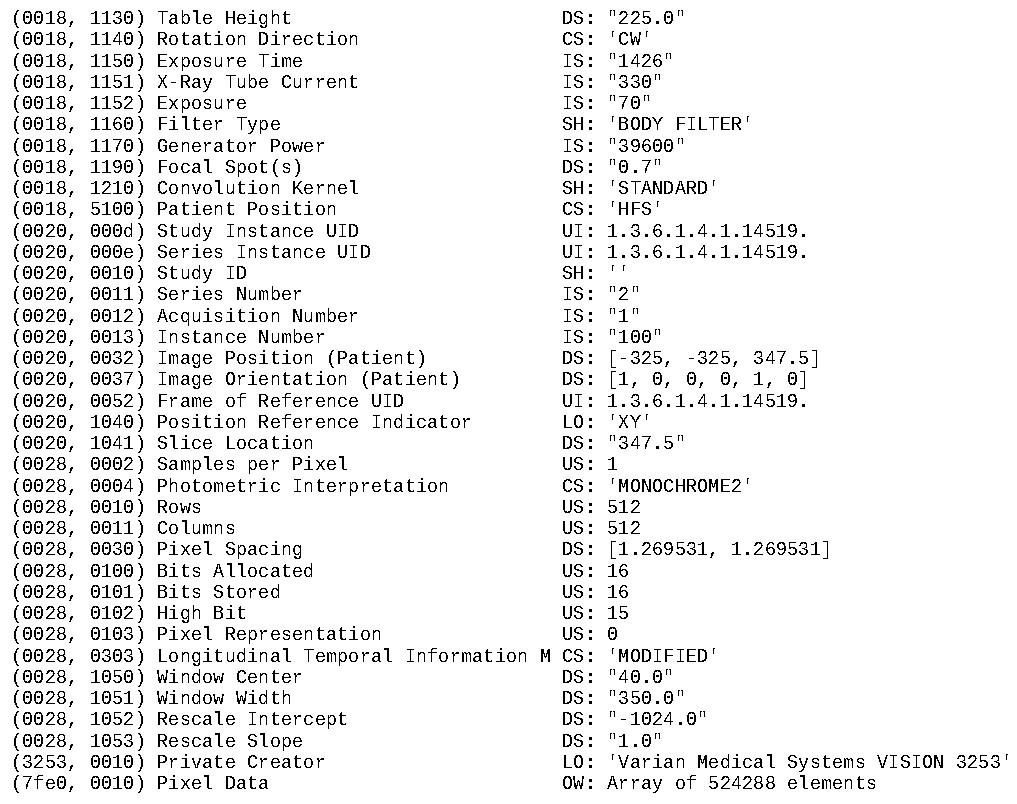
\includegraphics[width=\textwidth]{datasets/dicom.pdf}
  \caption[DICOM tags example]{DICOM file content example for a CT scan. On the left, DICOM tags which are tuples of two hexadecimal numbers, have an associated name to be readable by humans. On the right, the value of each DICOM tag is displayed. The \texttt{UID} tags values have been cut for readability.}
  \label{fig:dicom}
\end{figure}


\section{Lung Image Database Consortium image collection}
The first dataset that will be used in this work is the Lung Image Database Consortium image collection (LIDC-IDRI) dataset~\cite{armato_data_2015}. This dataset is the result of the collaboration of seven academic centers and eight medical imaging companies, under the initiation of the \emph{National Cancer Institute} (NCI), with the help of the \emph{Food and Drug Administration} (FDA) (United States). The goal of this collaboration and this dataset is "to develop, train and evaluate computer aided-diagnosis methods for lung cancer detection and diagnosis"~\cite{armato_lung_2011}.

The dataset contains three different types of scans: computed tomography (CT), digital radiography (DX) and computed radiography (CR) scans of the lungs. These scans cover about 1000 different patients, for a total of more than 240'000 images. All images in the dataset are in the DICOM format. In the LIDC-IDRI dataset, four radiologists have participated together to analyze and mark the whole set of CT scans. \citet{xie_transferable_2017} and \citet{ding_accurate_2017} have used this dataset for a detection task, while in this work it is used for a localization and a segmentation task (see Section~\ref{sec:lidcpreproc}).

The work of analysing this dataset has been separated in two different phases. During the first phase, the radiologists read all the CT scans in a blind manner, i.e. the radiologists have never seen the images before, and they do not know anything about the past history of the patients. Each radiologist was on his own, with no additional information, and had to mark the lesions and class them in three different categories:

\vbox{
  \begin{enumerate}
    \item Nodules >= 3 mm diameter
    \item Nodules < 3 mm diameter
    \item Non-Nodules >= 3 mm diameter
  \end{enumerate}}

For the first category, the radiologists drew the contour of this type of nodule in each slice of CT scan where the nodule appeared. Then, they were asked to subjectively give their opinion about some characteristics related to the nodule, for example the difficulty to detect the nodule, its internal structure, how well its margins are defined, or its malignancy. All characteristics are given in a scale between 1 and 5.

For the last two categories, the radiologists just gave the three-dimensional center of mass of these (non-)nodules.

\newpage
During the second phase, the results of the first phase were complied and send back to the four radiologists. They then read the marking work of the other radiologists. Finally, with the help of the four diagnoses, they were been asked to make a final decision about the marking and the characteristics.

All diagnoses, characteristics and annotations of the radiologists are stored in XML files. There is one XML file per CT series. An example of XML file for a nodule of the first category (Nodules >= 3 mm) is showed in the Listing~\ref{lst:lidcxml}. This example contains a nodule ID, the characteristics mentioned before, and the contour of the nodule, which is contained in the tag named \texttt{roi} (region of interest). The contour contains all the $x$ and $y$ coordinates of the points that make the contour of the nodule, and the universal identifier (UID) of the corresponding slice.

\lstinputlisting[float=t!, language=XML, caption={XML content example for a nodule >= 3 mm of the LIDC-IDRI dataset~\cite{armato_data_2015}. There is a nodule ID, some characteristics and a \texttt{roi} (region of interest) tag that contains the contour points $(x,y)$ of the nodule. The \texttt{imageSOP\_UID} tag has been left out for readability.}, label=lst:lidcxml, captionpos=b]{figures/datasets/lidcxml.xml}

\newpage
\section{Head-Neck-PET-CT dataset}
The second dataset that will be used in this work is the Head-Neck-PET-CT (HNPC) dataset~\cite{vallieres_data_2017}. It is a compilation of images, diagnoses and other medical information that are coming from four different institutions in Québec, Canada. 92 patients are coming from the \emph{Hôpital Général Juif} (HGJ) in Montréal, 102 from the \emph{Centre Hospitalier Universitaire de Sherbrooke} (CHUS), 41 patients from the \emph{Hôpital Maisonneuve-Rosemont} (HMR), and finally 65 from the \emph{Centre hospitalier de l’Université de Montréal} (CHUM).

The dataset contains computed tomography (CT) and positron emission tomography (PET) scans of the head, including the brain, to the neck. Both images types are given in the DICOM format. The HNPC dataset contains 300 different patients, that all have histologically proven head and neck cancer. The dataset contains a total of about 120'000 images. This patients data was used first in the work of \citet{vallieres_radiomics_2017}, that has been the trigger of the creation and compilation of the HNPC dataset.

The HNPC dataset contains, for each patient, several series. For each CT and PET scans series mentionned before, there is a corresponding radiotherapy structure set (RTStruct) series, that is a single DICOM file containing the contour points for several regions of interest (ROI) inside a DICOM tag. To illustrate, Figure~\ref{fig:hnpc_structset} shows a part of the \texttt{structure set ROI} DICOM tag, that contains ROI names and their correponding ROI number used further in the RTStruct, as a reference. The RTStruct file contains then, for each slice of its corresponding images series, the contour points of the ROIs and also a universal identifier that uniquely identifies the corresponding slice. These RTStruct series are the result of the work of radiologists coming from the four different institutions, that draw the contour of the ROIs, including tumors. The dataset contains also two other series named radiotherapy plan (RTPlan) and radiotherapy dose (RTDose). These two series contain more medical information about the patients, such as the planning of the therapy or the scheduling for the doses given to the patients.

With the HNPC dataset, two excel files are attached. The first of the two excel files is called \texttt{INFO\_clinical\_HN.xlsx} and contains textual medical information about all the patients, including for example the stage of the cancer, its primary location, the time of the diagnosis or the length of the treatment. In the second excel file, named \texttt{INFO\_GTVcontours\_HN.xlsx}, the gross tumor volume (GTV) names are listed under the same name as they appear in the RTStruct, as ROI name (see the DICOM tags \texttt{(3006,0026)} of the Figure~\ref{fig:hnpc_structset}).

\begin{figure}[t!]
  \centering
  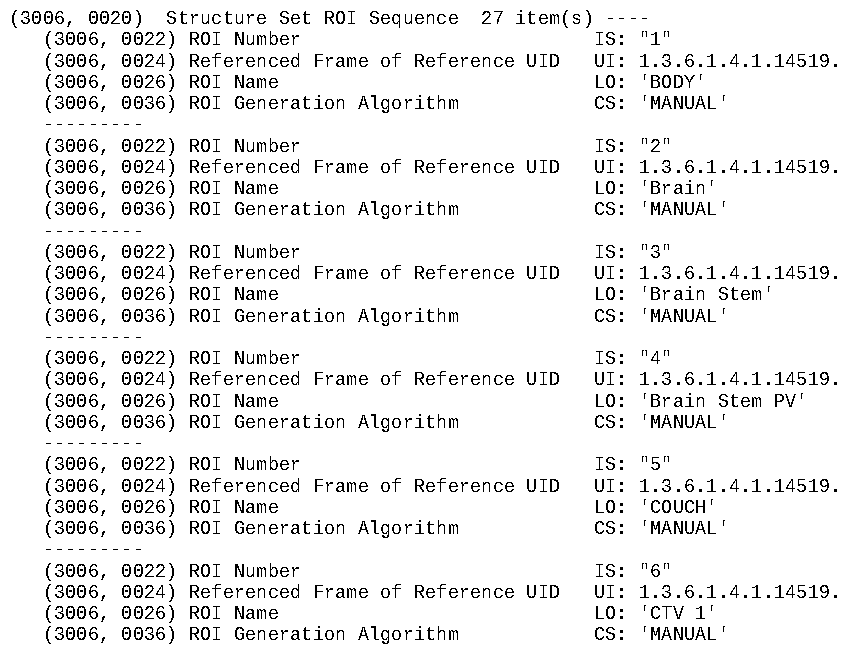
\includegraphics[width=\textwidth]{figures/datasets/hn_structsetroi.pdf}
  \caption[RTStruct DICOM content]{DICOM content example for an RTStruct series of the HNPC dataset~\cite{vallieres_data_2017}. DICOM tags can be seen on the left as tuples of two hexadecimal numbers, and their corresponding value can be seen on the right. The \texttt{UID} tags values have been cut for a better readability of the image.}
  \label{fig:hnpc_structset}
\end{figure}

\newpage
\section{Breast Ultrasound Images dataset}
The third and last dataset used in this work is the Breast Ultrasound Images (BUSI) dataset~\cite{al-dhabyani_dataset_2020}. This dataset is a collection of ultrasound images from the breast. The images were all collected in 2018, and they come from 600 different female patients, aged from 25 to 75. Originally, 1100 ultrasound images were collected at the \emph{Baheya hospital} in Egypt, under the DICOM format. Before constructing the dataset, radiologists have marked and reviewed annotations in the images.

The BUSI dataset contains, after reduction, a total of 780 ultrasound images, cropped and converted into the PNG format. The ground truth images, i.e. the segmentation masks, are given along the original images. These segmentation masks have been created by the radiologists over a year of work. For some images, there are more than one segmentation mask, if there is more than one tumor. The breast ultrasound images are separated in three categories: normal, benign and malignant. Each of these categories is a complete folder given in the dataset, containing images and their segmentation masks.

% !TEX root = ../main.tex

\chapter{Segmentation and preprocessing scripts}
\label{ch:preprocscripts}
This chapter presents the two core contributions of this work. First, a small introduction about the conversion of images is shown. The first main contribution is then explained. It consists of a new module that creates automatically the segmentation masks given the contour of a tumor. The second contribution is the preprocessing of the data itself. For each of the three datasets presented in the Chapter~\ref{ch:datasets}, the preprocessing is explained in detail. All code is written in the Python programming language and publicly available on GitHub\footnote{\url{https://github.com/ChristopheBroillet/Hydra_Segmentation}}.

\section{Images conversion}
\label{sec:imgconversion}
In computer science, images are stored as tables of numbers. Each cell in the table corresponds to one pixel in the image, and contains a certain value (number) that represents the pixel intensity, i.e. the strength of the pixel in a the given type of image. An image can have one or more channels, i.e. layer of pixels, that are stacked to form the image. Three of the most used types of image are:
\begin{enumerate}
  \item The \emph{monochrome image}, also called binary image, contains a binary intensity that is either on or off, and can be interpreted as black and white image. The pixels have either the value 0 (black) or the value 1 (white). The monochrome image is thus encoded in 1 bit per pixel, and has only one channel.
  \item The \emph{greyscale image} contains only intensities on a grey scale. The difference with the monochrome image is that the grey color has many shades and not only 2. The pixel intensity represents then the level of grey of the pixel, and the value depends on the encoding. For example, if a greyscale image is encoded in 8 bits per pixel, the range of the pixel intensity will be $[0,255]$. Here, the black pixel corresponds to the value 0 and the white to the 255 value. The greyscale image has also only one channel.
  \item The \emph{red green blue (RGB) image} is a color image. To represents the colors, shades of red, green and blue are added. The pixel intensity depends on the encoding too. The RGB image contains 3 channels, one for the red, one for the green and one for the blue. These 3 channels are then stacked to form the RGB image. In that case, a pixel is not represented by only one value, as in the two previous types, but by a tuple of three values, one for each RGB colors.
\end{enumerate}

As stated in Section~\ref{sec:dicom}, the DICOM standard aims to standardize all medical images and data between medical institutions worldwide. DICOM converts images with information contained in DICOM tags. The conversion described below is applied on the \texttt{pixel data (7fe0,0010)} DICOM tag, that contains one or more medical images, and will result in converted output images. The conversion is done in two steps that are explained below, while the corresponding code of this work is written in the \texttt{normalize\_dicom} module available on GitHub\footnote{\url{https://github.com/ChristopheBroillet/Hydra_Segmentation/blob/main/preprocessing_scripts/Head-Neck-PET-CT/normalize_dicom.py}}.

\subsection{Hounsfield correction}
The \emph{Hounsfield units} (HU) are universally used units in CT or PET scans, to display a standardized image. The Hounsfield scale is based on the measure of the radiodensity, i.e. the ability of electromagnetic waves to go through a given material. The arbitrarily defined radiodensity of the distilled water (at standard temperature and pressure) is 0~HU, while radiodensity of air is -1000~HU~\cite{schneider_calibration_1996}.

To convert a CT or PET scan, the raw data pixels are first converted using the Hounsfield correction. The equation used to convert original data to HU is given by:
\begin{equation}
  HU = m \cdot P + b
\end{equation}
where $HU$ is the output value in Hounsfield unit, $m$ is the rescale slope given in the \texttt{rescale slope (0028,1053)} DICOM tag, $P$ the input value of the pixel and $b$ the rescale intercept given in the \texttt{rescale intercept (0028,1052)} DICOM tag.

The use of the Hounsfiels units have helped radiologists to interpret and diagnose disease on CT or PET scans. Indeed, scanners take images that have in principle between 12 and 16 bits per pixel, that is between 4096 to 65536 shades of grey. But human eyes struggle to distinguish this amount of shades, while medical displays support encodings from 8 to 10 bits per pixel nowadays. To avoid these two problems, CT and PET scans are converted using the Hounsfield units~\cite{kimpe_increasing_2007}.

\subsection{Normalization}
After this first correction in HU, another linear transformation needs to be applied. This second transformation is necessary in order to keep a normalized output range value $[y_{min},y_{max}]$ for the pixels. To get this output range, the following rules\footnote{These rules are taken from the DICOM standard browser: \\ \url{https://dicom.innolitics.com/ciods/ct-image/voi-lut/00281050}} will be applied to the resulting $HU$ from the first correction for CT and PET scans. For other modalities, they will be applied directly on the pixel values of the image:
\begin{align}
  \begin{split}
    \text{if } HU &\leq c - 0.5 - \dfrac{w - 1}{2} \text{, then } y = y_{min} \\
    \text{else if } HU &> c - 0.5 + \dfrac{w - 1}{2} \text{, then } y = y_{max} \\
    \text{else } y &= \left( \dfrac{HU - (c - 0.5)}{w - 1} + 0.5 \right) \cdot (y_{max} - y_{min}) + y_{min}
  \end{split}
\end{align}
with $HU$ the input pixel value, $c$ the window center given in the \texttt{window center (0028,1050)} and $w$ the window width in the \texttt{window width (0028,1051)}, $y_{min}$ and $y_{max}$ the minimum and maximum value of the output range, and $y$ the output value.

In this work, the output range value will be $[0,255]$, as the output image will be a greyscale image with 8 bits per pixel. In this case, $y_{min} = 0$ and $y_{max} = 255$.


\section{The \texttt{segmentation\_mask} module}
\label{sec:segmaskmodule}
In this work, a new module is provided: the \texttt{segmentation\_mask} module. The goal of this module is to create a segmentation mask for a medical image, given the contour points of the segmentation of the tumor. These contour points are given as ground truth with the dataset they belong to. With these segmentation masks, the deep learning model can be fed with both medical images and segmentation masks. As explained in the Section~\ref{sec:deeplearning}, the medical images are the inputs of the network and the segmentation masks are the labels. The \texttt{segmentation\_mask} module contains two new functions described in the following paragraphs.

\subsection{The \texttt{mm\_to\_imagecoordinates} function}
\label{sec:mmtocoord}
In some cases, like in the Head-Neck-PET-CT dataset, the segmentation points are given in the Patient-Based Coordinate System (PBCS), that are in absolute distance given in millimeters within the patient body. The PBCS is a 3D orthonormal right-handed system, i.e. where the cross product of a unit vector along a $x$ axis and $y$ unit vector gives a $z$ unit vector. Figure~\ref{fig:pbcs} shows one of the most used PBCS orientation.

\begin{figure}[t!]
  \centering
  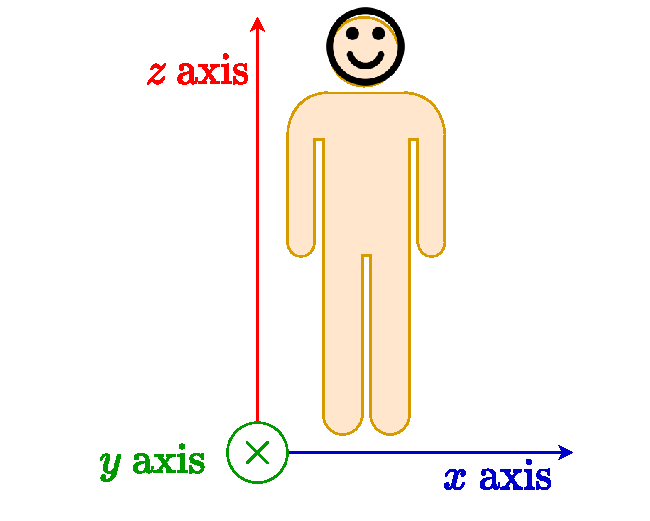
\includegraphics[height=0.25\textheight]{preprocscripts/pbcs.pdf}
  \caption[Patient-base coordinate system orientation example]{Example of an orientation of the patient-base coordinate system. The $x$ axis points from the right to the left of the patient, the $y$ axis from the face to the back of the patient (the axis enters the plane) and the $z$ axis points from the feet to the head of the patient.}
  \label{fig:pbcs}
\end{figure}

The preprocessing and conversion of the images need the row and column indices of the image. The first function of the module, called \texttt{mm\_to\_imagecoordinates}, is used to convert units from the PBCS given in mm, to the image plane coordinate system (IPCS) given in indices. The formula that will be used to convert from one system to the other is taken from the DICOM standard browser\footnote{\url{https://dicom.innolitics.com/ciods/ct-image/image-plane/00200032}}:
% \newpage
\begin{equation}
\label{eq:mmToIndicesMatrix}
  \begin{bmatrix}
    P_x \\ P_y \\ P_z \\ 1
  \end{bmatrix} =
  \begin{bmatrix}
    X_x \Delta_i & Y_x \Delta_j & 0 & S_x \\
    X_y \Delta_i & Y_y \Delta_j & 0 & S_y \\
    X_z \Delta_i & Y_z \Delta_j & 0 & S_z \\
    0 & 0 & 0 & 1 \\
  \end{bmatrix}
  \begin{bmatrix}
    i \\ j \\ 0 \\ 1
  \end{bmatrix}
\end{equation}

The point $(P_x, P_y, P_z)$ represents the coordinates of the point along the three $x,y,z$ axis in the PBCS. It is the point that will be converted in the IPCS. The point given by $(S_x, S_y, S_z)$ is the upper-left pixel in the PBCS, that will be the origin $(0,0,0)$ of the converted image in the IPCS. It is contained in the \texttt{image position (patient) (0020,0032)} DICOM tag. Then, the DICOM tag \texttt{image orientation (patient) (0020,0037)} gives the $(X_x, X_y, X_z, Y_x, Y_y, Y_z)$ values. The $(X_x, X_y, X_z)$ are the direction cosines (i.e. cosines of angles) between the $x$ axis of the Figure~\ref{fig:pbcs} and the row direction of the IPCS. It expresses the change of direction in the PBCS when moving from one column to the next in the IPCS. Similarly, the $(Y_x, Y_y, Y_z)$ are the direction cosines between the $y$ axis of the Figure~\ref{fig:pbcs} and the column direction of the IPCS, and it expresses the change of direction in the PBCS when moving from one row to the next in the IPCS. For example, if the orientation of the PBCS is exactly the one presented in the Figure~\ref{fig:pbcs}, then $(X_x, X_y, X_z, Y_x, Y_y, Y_z)$ will be equal to $(1,0,0,0,1,0)$. Further, the \texttt{pixel spacing (0028,0030)} DICOM tag gives the column spacing $\Delta_i$ between the center of two adjacent pixels in mm, and $\Delta_j$ the row spacing. Finally, $i$ is the \emph{column} index and $j$ the \emph{row} index of the converted image.

As images are in two dimensions, the first two equations of~\eqref{eq:mmToIndicesMatrix} are:
\begin{equation}
  \label{eq:mmToIndicesAlgebra}
  \begin{cases}
    P_x = X_x \Delta_i i + Y_x \Delta_j j + S_x \\
    P_y = X_y \Delta_i i + Y_y \Delta_j j + S_y
  \end{cases}
\end{equation}

The \texttt{solve} method of the \texttt{linalg} module provided by \texttt{NumPy}~\cite{harris_array_2020} is used to solve this system of two equations for $i$ and $j$. The next described function uses the presented function in an optional manner. If the contour points are given in the PBCS, the script needs to call this method to convert the points. If the contour points are already given in the IPCS, then no conversion is required.


\subsection{The \texttt{create\_segmentation\_mask} function}
The second and main function of this module is the \texttt{create\_segmentation\_mask} function. Indeed, this is the function that is primarily called in the preprocessing scripts to start the creation of the segmentation masks. To open and use DICOM files in Python, this function uses the \texttt{pydicom} library~\cite{mason_su-e-t-33_2011}. The outputed segmentation masks are monochrome images. Indeed, black pixels (value 0) represent no tumor, while white pixels (value 1) represent tumor. As arguments, the function takes:
\begin{itemize}
  \item The data contour points of the segmentation. The data needs to be a 2D list, i.e. a list of points $(x,y)$ of the segmentation. The data is considered as ground truth.
  \item The medical image slice that corresponds to the segmentation. This is an opened DICOM file from the \texttt{pydicom} library.
  \item The path to an output folder. This folder will contain the outputed segmentation masks.
  \item A boolean called \texttt{conversion} that indicates if the conversion is required or not. If \texttt{conversion} is \emph{True}, the \texttt{create\_segmentation\_mask} function will use the previous described function in Section~\ref{sec:mmtocoord}.
\end{itemize}
Algorithm~\ref{algo:createsegmask} shows in pseudocode the different steps to create the segmentation masks, by calling the \texttt{create\_segmentation\_mask} function. The following paragraphs explain those steps in detail.

\begin{algorithm}[t!]
  \caption{\texttt{create\_segmentation\_mask} function}
  \label{algo:createsegmask}
  \begin{algorithmic}[1]
    \Function{create\_segmentation\_mask}{$img, data, output\_folder, conversion$}
    \State Create a $log\_file$ \Comment \texttt{.txt} file
    \State Initialize $seg\_mask \gets img \cdot 0$ \Comment 0 for black pixels
    \For{each $point$ in $data$}
      \If{$conversion$} \Comment $conversion$ is a boolean
        \State $x, y \gets$ \texttt{mm\_to\_imagecoordinates}$(img, point)$
      \Else
        \State $x, y \gets point$
      \EndIf
      \State $seg\_mask[y][x] \gets 1$ \Comment Add white pixel
    \EndFor
    \State Initialize $white\_boundaries$\Comment Will contain white indices for each row
    \For{each $white\_row$ in $seg\_mask$}
      \State $white\_boundaries$ append $[row\_idx, min\_white\_idx, max\_white\_idx]$
    \EndFor
    \State Sort $white\_boundaries$ by $row\_idx$
    \State \Comment Two rows at a time, row counter incremented by 1 at each iteration
    \For{each $first, second$ in $white\_boundaries$}
      \If{$first$ and $second$ not differ by 1 in their indices} \Comment Missing line
        \State Add missing line with average value of $first$ and $second$
        \State Write entry in $log\_file$
      \EndIf
    \EndFor
    \State \Comment Three rows at a time, row counter incremented by 1 at each iteration
    \For{each $first, second, third$ in $white\_boundaries$}
      \State $average \gets average(first, second)$
      \State Define $ERROR\_THRESHOLD = 0.05$ \Comment Tolerate to 5\% error
      \If{$\left| \frac{average - second}{average} \right| > ERROR\_THRESHOLD$} \Comment Absurd value
        \State $second \gets average$
        \State Write entry in $log\_file$
      \EndIf
    \EndFor
    \State Sort $white\_boundaries$ by $row\_idx$
    \State Fill white rows in $seg\_mask$ according $white\_boundaries$
    \State \Return{$seg\_mask$}
    \EndFunction
  \end{algorithmic}
\end{algorithm}

At first, an empty mask is initialized, with all pixels value to be 0 (black pixels). This mask will have the same size as the medical image. Then, the contours points given as argument of the function are drawn on the mask as white pixels (value 1). At the same time, a simple log file is created to keep track of the modifications and potential errors occuring during the second step.

The data contour points given with datasets can be partially missing or wrong. Indeed, data is entered by humans and can be the source of mistakes. Data transmission between medical institutions, as well as digitization of old data can also lead to errors. During the second step, the data of the contour points is thus imputed and mitigated if necessary. The presented module first proceeds to imputation, i.e. looks at missing data. It checks if there is a missing line among the contour by looking at the row indices of two consecutive lines. If a line is missing, it looks at the neighbour lines and compute their average white boundaries. The white boundaries delimit the section of a row that contains white pixel. Finally, an entry in the log file is added, specifiying which line was missing.

After imputation of the data, i.e. completing the potential missing rows, the function will then start a data mitigation process, to look for absurd values. It will look at three rows at a time for each iteration step, and compute the average value of the first and third line. This computed value will then be compared with the value of the second (middle) line. If the comparison results in a too big difference between the values, defined by a threshold, the middle value is considered as an error or an absurd value. In this work, a too big difference (absurd value) is when values of white boundaries differ from more than 5\% than their neighbours. The data is then mitigated by replacing the old value with the neighbour average value, and an entry is added to the log file, with the old and new values.

Figure~\ref{fig:segmasklog} shows an example log file for an image of the HNPC dataset. The HNPC contained some missing lines and absurd values in the data extracted from the RTStruct series, while the LIDC-IDRI dataset had no errors.

\begin{figure}[t!]
  \centering
  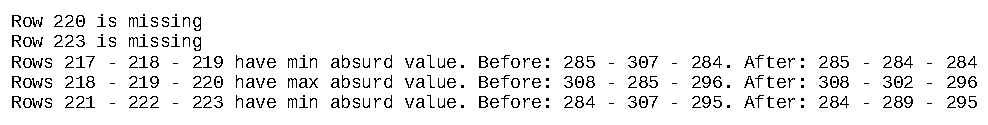
\includegraphics[width=\textwidth]{preprocscripts/segmasklog.pdf}
  \caption[Example log file from the \texttt{create\_segmentation\_mask} function]{Example log file from the \texttt{creste\_segmentation\_mask} function. This file tells the user that the rows 220 and 223 were missing in the original data, and were added by the function. Then, the function mitigated some values that had more than 5\% error. The file shows the old and new values.}
  \label{fig:segmasklog}
\end{figure}

The following sections will present and explain the preprocessing Python scripts for the new datasets, in both textual information or in pseudocode. To manage the DICOM files contained in the datasets but also to get the access to the DICOM tags, the scripts will use the \texttt{pydicom} library.

\section{LIDC-IDRI preprocessing}
\label{sec:lidcpreproc}
In order to use this dataset for a supervised learning training purpose, the images and the medical diagnoses have to be preprocessed first. Because of simplicity and completeness of the data and their labels in the dataset, this work only considers the first category (Nodules >= 3 mm). The other two categories are left out.

The LIDC-IDRI dataset can be used for two different tasks. The first task will be the \emph{localization} task, to detect if the nodules are cancerous or not, and also locate them within the image. The second task will be the \emph{segmentation} task, where the contour of the cancerous nodule will be drawn. The preprocessing is done in a single step, where the images are converted from DICOM to \texttt{NumPy} arrays, and the labels are collected. For each slice, the label for the localization task will be a True/False diagnosis and the location of the center of the nodule, as the label for the segmentation task will be a segmentation mask. For the preprocessing of this dataset, only one script has been written. When running it, the user is first asked to enter the task he wants to perform, either the localization or the segmentation. The script then performs the given task.

\subsubsection{Preprocessing for the localization task}
The idea of the preprocessing for the localization is to first classify in a binary manner the nodules according their malignancy, given in a 1 to 5 scale by the radiologists, 1 being benign and 5 being malignant. The nodules that have a malignancy of 1 or 2 are treated as False cases, while the nodules with a malignancy of 4 or 5 are treated as True cases. The nodules with malignancy 3 are left aside as the diagnosis is uncertain.

Then, for each of this cases, the corresponding slice is searched and taken. As the contour is given in a XML file for each of these slices, the $x$ and $y$ coordinates are extracted, and the center of the nodule is computed, via a mean calculation. The slices are finally converted into greyscale images encoded in 8 bits per pixel (pixel intensity from 0 to 255) using the conversion steps of Section~\ref{sec:imgconversion}. The script does this conversion so that the slice can be displayed correctly on a screen. The center of the nodule is saved in the name of the file, and the True and False cases are separated in two different output folders. For example, a True case can have the name \texttt{LIDC-IDRI-0001\_nid-0\_pos-314-365\_29.npy}. The first part, \texttt{LIDC-IDRI-0001} is the patient ID, \texttt{nid-0} is the nodule ID as the case can have more than one nodule. Then, the position of the center of the nodule \texttt{pos-314-365} is given in $(x,y)$ coordinates. Finally, the last number \texttt{29} is an added index to avoid duplicate names. The different steps to preprocess the dataset for the localization are shown in the Algorithm~\ref{algo:lidcpreproclocalization}.

\begin{algorithm}[t!]
  \caption{LIDC-IDRI preprocessing for the \emph{localization} task}
  \label{algo:lidcpreproclocalization}
  \begin{algorithmic}[1]
    \State Create two folders $True$ and $False$ in $output\_folder$
    \For{each $series$ in $dataset\_folder$} \Comment{Iterate over patients/studies/series}
      \If{$series$ is not CT}
        \State Continue
      \EndIf
      \State Initialize $nodules\_df['Nodule ID', 'x pos', 'y pos', 'z pos', 'Diagnosis']$
      \State Get the 4 $reading\_sessions$ of the radiologists \Comment{By parsing XML file}
      \For{each $session$ in $reading\_sessions$}
        \For{each $nodule$ in $session$}
          \If{malignancy in [1,2]}
            \State $diagnosis = False$
          \ElsIf{malignancy in [4,5]}
            \State $diagnosis = True$
          \Else
            \State Continue
          \EndIf
          \State Initialize $x\_coords = []$ and $y\_coords = []$
          \For{each $slice$ in $nodule$}
            \For{each $contour\_point$ in $slice$}
              \State $[x, y] \gets contour\_point$ \Comment{Get coordinates}
              \State $x\_coords$ append $x$
              \State $y\_coords$ append $y$
            \EndFor
            \State $x\_mean \gets mean(x\_coords)$
            \State $y\_mean \gets mean(y\_coords)$
            \State $z \gets slice$
            \State $nodules\_df$ append $[NoduleID, x\_mean, y\_mean, z, Diagnosis]$
          \EndFor
        \EndFor
      \EndFor
      \For{each $row$ in $nodules\_df$}
        \For{each $dicom\_image$ in $patient$}
          \If{$dicom\_image$ is the slice where the nodule of $row$ appears}
            \State $diagnosis \gets row['Diagnosis']$
            \State $slice \gets normalize(dicom\_image)$ \Comment{\texttt{normalize\_dicom} module}
            \State Save $slice$ in $output\_folder/\{diagnosis\}$
          \EndIf
        \EndFor
      \EndFor
    \EndFor
  \end{algorithmic}
\end{algorithm}

\subsubsection{Preprocessing for the segmentation task}
The preprocessing for the segmentation task is very similar to the preprocessing for the localization task, as it uses the same dataset. The script for the localization task took the nodules of the first category (Nodules >= 3 mm) with malignancy 1, 2, 4 or 5. For the segmentation however, the script only takes the cancerous nodules, i.e. with malignancy 4 or 5. The other ones are left out.

Then, the XML parsing is done in the very same way as the localization task, by getting all contour points, but this time the center of the nodules is not computed, as only the contour points themselves are required to do the segmentation task. These contour points are then saved in a list.

Finally, the images are converted into greyscale images encoded in 8 bits per pixel, and the segmentation masks, that are monochrome images, are created using the \texttt{segmentation\_mask} module. Algorithm~\ref{algo:lidcpreprocsegmentation} shows the steps to preprocess the dataset for the segmentation task.

\begin{algorithm}[t!]
  \caption{LIDC-IDRI preprocessing for the \emph{segmentation} task}
  \label{algo:lidcpreprocsegmentation}
  \begin{algorithmic}[1]
    \State Create two folders $img$ and $masks$ in $output\_folder$
    \For{each $series$ in $dataset\_folder$} \Comment{Iterate over patients/studies/series}
      \If{$series$ is not CT}
        \State Continue
      \EndIf
      \State Initialize $nodules\_df['Nodule ID', 'contour data', 'z pos']$
      \State Get the 4 $reading\_sessions$ of the radiologists \Comment{By parsing XML file}
      \For{each $session$ in $reading\_sessions$}
        \For{each $nodule$ in $session$}
          \State Select nodules of malignancy $\geq 4$
          \State Initialize $contour\_points = []$
          \For{each $slice$ in $nodule$}
            \For{each $contour\_point$ in $slice$}
              \State $[x, y] \gets contour\_point$ \Comment{Get coordinates}
              \State $contour\_points$ append $[x, y]$
            \EndFor
            \State $z \gets slice$
            \State $nodules\_df$ append $[NoduleID, contour\_points, z]$
          \EndFor
        \EndFor
      \EndFor
      \For{each $row$ in $nodules\_df$}
        \For{each $image$ in $patient$}
          \If{$image$ is the slice where the nodule of $row$ appears}
            \State $image\_slice \gets normalize(image)$ \Comment{\texttt{normalize\_dicom} module}
            \State Save $image\_slice$ in $output\_folder/img$
            \State $segmentation\_mask \gets create\_segmentation\_mask$
            \State Save $segmentation\_mask$ in $output\_folder/masks$
          \EndIf
        \EndFor
      \EndFor
    \EndFor
  \end{algorithmic}
\end{algorithm}

\newpage
\section{HNPC preprocessing}
The preprocessing of the Head-Neck-PET-CT dataset is separated in two phases. In the first phase, the preprocessing script iterates over all patients, studies and series. It then checks the modality of the series. If the series is a CT or PET series (image series) or a RTStruct series, the script continues. If the modality is something else, like RTDose or RTPlan, the series is just skipped as the script does not need it to preprocess for the segmentation task.

Then, the script reads the spreadsheet \texttt{INFO\_GTVcontours\_HN.xlsx}, and extracts the names the radiologists gave to the tumors. For both types of image series (CT and PET), the script saves the Patient ID, the series universal identifier (UID), the modality, the path and the roi name of the tumor in a \texttt{pandas}~\cite{the_pandas_development_team_pandas-devpandas_2020, mckinney_data_2010} dataframe. In addition, for the RTStruct series only, the script also saves the series UID of its referenced image series. In that way, the dataframe contains names, UID and relations between the RTStruct series and their corresponding images. This will make it easier to work with in the next step.

In the second phase, the \texttt{pandas} dataframe just created is separated in two other dataframes: one containing only the images series, and the other containing the \mbox{RTStruct} series. An iteration is then started in the RTStruct dataframe. The goal of this iteration is to first take the RTStruct and its corresponding images series, and for each slice of the images series that contains the tumor, it then extracts the contour points that segment the tumor. Finally, the image is as before converted into a \texttt{NumPy} array, and the contour points are inputed into the \texttt{segmentation\_mask} module, which outputs the segmentation mask. The Algorithm~\ref{algo:hnpcpreproc} shows all this preprocessing.

\begin{algorithm}[t!]
  \caption{HNPC preprocessing}
  \label{algo:hnpcpreproc}
  \begin{algorithmic}[1]
    \State Create two folders $img$ and $masks$ in $output\_folder$
    \State Initialize $metadata\_df$
    \State Read excel file $roinames\_excel$ \Comment{\texttt{INFO\_GTVcontours\_HN.xlsx}}
    \For{each $patient$ in $dataset\_folder$}
      \For{each $visit$ in $patient$}
        \For{each $series$ in $visit$}
          \If{$series$ is CT, PET or RTStruct}
            \State $metadata\_df$ append metadata information
          \EndIf
        \EndFor
      \EndFor
    \EndFor
    \State Split $metadata\_df$ in $RT\_df$, $images\_df$ \Comment according to modality
    \For{each $row$ in $RT\_df$}
      \State $dicom\_file \gets row$
      \State Open $dicom\_file$ \Comment{Get $ROI\_contour\_sequence$}
      \For{each $contour\_sequence$ in $ROI\_contour\_sequence$}
        \State $contour\_image \gets contour\_sequence[0\text{x}3006,0\text{x}16][0]$ \Comment{DICOM tag}
        \State $series\_images\_path \gets contour\_image[0\text{x}8,0\text{x}1155].value$ \Comment{DICOM tag}
        \For{each $image$ in $series\_images\_path$}
          \State $dicom\_image \gets$ Search the referenced slice
          \State $image\_slice \gets normalize(dicom\_image)$ \Comment{\texttt{normalize\_dicom} module}
          \State Save $image\_slice$ in $output\_folder/img$
          \State $segmentation\_mask \gets create\_segmentation\_mask$
          \State Save $segmentation\_mask$ in $output\_folder/masks$
        \EndFor
      \EndFor
    \EndFor
  \end{algorithmic}
\end{algorithm}

\newpage
\section{BUSI preprocessing}
The preprocessing steps of BUSI are much shorter than in the two previous datasets. As the images are given in the PNG format, the preprocessing script does no use the \texttt{pydicom} library. While the segmentation masks have already been created and given in the dataset, the script does not use either the \texttt{segmentation\_mask} module. No resizing or rescaling operation is needed, as images and masks are already in the same size. Thus, a simple conversion from PNG to \texttt{NumPy} array is required to preprocess this dataset. As the segmentation masks for the images of the first category (normal) are empty, this category is not taken in the preprocessing.

For both remaining categories (benign and malignant), the preprocessing script iterates over the original images. It can then find the corresponding segmentation masks, as they have the same name as the images. Once the image and its mask are found, they are converted into \texttt{NumPy} arrays, in format of 8 bits per pixel, 1-channel greyscale. They are finally saved under two distinct folders, one for the images and one for the masks. The preprocessing of the BUSI dataset is already finished. The Algorithm~\ref{algo:busipreproc} shows the different steps to preprocess the BUSI dataset.

\begin{algorithm}[t!]
  \caption{BUSI preprocessing}
  \label{algo:busipreproc}
  \begin{algorithmic}[1]
    \State Create two folders $img$ and $masks$ in $output\_folder$
    \For{each $category$ in $dataset\_folder$}
      \If{$category = normal$}
        \State Continue
      \EndIf
      \State $image\_paths\_list \gets$ Get all original images of $category$
      \For{$image\_path$ in $image\_paths\_list$}
        \If{$image\_name$ matches $image\_path$} \Comment With a RegEx
          \State Construct $mask\_name$ and $mask\_path$ from $image\_name$
          \State $image\_slice \gets convert(image\_path)$
          \State Save $image\_slice$ in $output\_folder/img$
          \State $segmentation\_mask \gets convert(mask\_path)$
          \State Save $segmentation\_mask$ in $output\_folder/masks$
        \EndIf
      \EndFor
    \EndFor
  \end{algorithmic}
\end{algorithm}


\section{Discussion}
This work improves the Hydra framework in the following ways:
\begin{itemize}
  \item The new \texttt{segmentation\_mask} module provides a robust way to create segmentation masks, given a medical image and the contour points of the tumor. The module is ready to be used for other future datasets for the segmentation task, and will give the segmentation masks for each image. Even if the contour points data is not complete or have some absurd values, the module will impute and mitigate the missing data. The \texttt{segmentation\_mask} outputs two different files. On one hand, the segmentation masks that are monochrome images, will represent the labels during the training of Hydra, in a supervised learning manner. On the other, each mask will have a proper log file containing information about the imputation and mitigation of the data if necessary. The user can check these log files for a debugging purpose, and to see where data contained errors. Finally, the proper segmentation mask is created and returned along with the preprocessed medical image.
  \item The \texttt{segmentation\_mask} module can also be used to segment other objects than just tumors. For example, if a CAD system is designed to segment the prostate itself as in the \emph{PROMISE12} challenge (see Section~\ref{sec:cadsegtask}), then this module is ready to output a mask that segments the prostate, and can be easily added to this CAD system.
  \item Hydra can now uses new datasets. Indeed, after all the preprocessing steps presented in this work that are implemented in three different preprocessing scripts, the three datasets are now ready to be used to train the Hydra model. Firstly, the \emph{lung image database collection} can be used either for the localization task, or the segmentation task. A single script preprocesses this dataset for the two tasks. Then, the \emph{head-neck-PET-CT} and the \emph{breast ultrasound images} datasets can both be used for the segmentation task. At the end, each medical image has its own corresponding segmentation mask as ground truth, and they can be used together to train the segmentation task in a supervised learning manner.
  \item The \texttt{normalize\_dicom} has received some minor changes. The code has been cleaned to be more readable by the user, but it basically achieves the same goal: convert the medical images in a standardized manner, with or without the use of the Hounsfield units, and in a way that Hydra can read.
\end{itemize}

% !TEX root = ../main.tex

\chapter{Conclusion}
\label{ch:conclusion}

This work presented the new contributions on a computer aided diagnosis (CAD) system named Hydra, that can detect cancerous tumors. The Hydra framework was born under a collaboration between the H-FR and the eXascale Infolab of the University of Fribourg. This work contributes three scripts that preprocess three new datasets: they modify and transform the data so that it can be used with the Hydra model. The number of datasets for the Hydra framework has been doubled. With these new datasets, this work helps avoiding the problem of scarcity of publicly available medical data.

Another contribution of this work is also the implementation of a new task for the CAD system, named the segmentation. This was possible by developing a brand new module. It creates a segmentation mask given a medical image and a list of contour points that delimit the tumor. The new module has been used on three new datasets: two of them are preprocessed for the segmentation task while the last one is preprocessed for both localization and segmentation tasks.


\section{Future Work}
As the new module that creates the segmentation masks has been developed in this work and is ready to be used, the next goal is to utilize it in the Hydra framework. That means, a new Hydra model has to be constructed on purpose for segmentation task. A model that is used nowadays for segmentation is the U-Net architecture~\cite{navab_u-net_2015}. Hydra can then use this U-Net model instead of the current VGG-16 model.

Another way to improve Hydra's performance is to augment the data already preprocessed in this work: by flipping or rotating for example, the medical images are not the same to the eyes of the machine, and thus will extend the data available for the Hydra framework.

In the next years with improvement and advent of new machine learning techniques, the Hydra framework or other CAD systems will hopefully be used to really help radiologists to detect as early as possible the first stages of cancer, resulting in saving human lives.



%----------------------------------------------------------------------------------------
%	BIBLIOGRAPHY
%----------------------------------------------------------------------------------------
\printbibliography[heading=bibintoc]


%----------------------------------------------------------------------------------------
%   APPENDIX
%----------------------------------------------------------------------------------------
% Rarely required, only if extra material particularly voluminous
% % !TEX root = ../main.tex

\chapter{Frequently Asked Questions} % Main appendix title
\label{ch:appendix}

\section{How do I change the colors of links?}

The color of links can be changed to your liking using:

{\small\verb!\hypersetup{urlcolor=red}!}, or
{\small\verb!\hypersetup{citecolor=green}!}, or
{\small\verb!\hypersetup{allcolor=blue}!}.
\noindent If you want to completely hide the links, you can use:
{\small\verb!\hypersetup{allcolors=.}!}, or even better:
{\small\verb!\hypersetup{hidelinks}!}.
\noindent If you want to have obvious links in the PDF but not the printed text, use:
{\small\verb!\hypersetup{colorlinks=false}!}.



%----------------------------------------------------------------------------------------
\end{document}
% That's all folks
